% slides_example.tex
%
% Example .tex file for the beamer-purdue theme
%
% Copyright (c) 2018 Dennis Ogbe <dogbe@purdue.edu>
%
% This file is published under the Creative Commons Attribution 4.0
% International License. For more information, please visit
% https://creativecommons.org/licenses/by/4.0/
%
% See the README.md for usage instructions. This style really only has one
% option: When called with the "altlogo" option, it will use the "Purdue
% University" logo instead of the "Purdue Engineering" logo.

% 16:9 aspect ratio for modern displays
\documentclass[pdf,smaller,aspectratio=169]{beamer}
%\documentclass[pdf,smaller,aspectratio=43]{beamer} % 4:3 for traditional beamer feel
\usepackage[utf8]{inputenc}

% switch to presentation mode
\mode<presentation>{}

% load required packages. I prefer IEEEtran for equations, but that's a
% personal preference.
\usepackage{IEEEtrantools}
\usepackage[cmex10]{mathtools} % for math equations
\usepackage{amsthm}
\usepackage{amssymb}
\usepackage{bm}
\usepackage{verbatim}

% demo for transparent full-frame background images
\usepackage[export]{adjustbox}

% theorems - can use \begin{IEEEproof} as alternative to \begin{proof}
\renewcommand{\qedsymbol}{$\blacksquare$} % want a black square for proofs

% useful to set this when using Inkscape SVG figures
\graphicspath{{./graphics/}}

% use the off-white theme
\usetheme{framed}

% demo of references with biber/biblatex -- recommended to get the right look and functionality (footfullcite etc)
\usepackage{filecontents}
\begin{filecontents}{refs.bib}
@ARTICLE{shannon48,
author={C. E. {Shannon}},
journal={The Bell System Technical Journal},
title={A mathematical theory of communication},
year={1948},
volume={27},
number={3},
pages={379-423},
keywords={},
doi={10.1002/j.1538-7305.1948.tb01338.x},
ISSN={0005-8580},
month={July},}
\end{filecontents}

\usepackage[bibstyle=ieee,citestyle=numeric,backend=biber]{biblatex}
\addbibresource{refs.bib}
\defbibheading{bibliography}[\bibname]{}

% set the purdue seal as title graphic and logo on the slides
% This is the purdue seal. use scalebox or resizebox to fit it in. the argument is the color in which it will be drawn
%
% Converted from SVG to TikZ by Dennis Ogbe <dogbe@purdue.edu>
\newcommand{\purdueseal}[1]{%
  \begin{tikzpicture}[yscale=-1,inner sep=0pt, outer sep=0pt,fill=#1]
    \path[fill] (80.4740,6.9590) .. controls (80.5560,7.0260) and (80.4210,7.2440) ..  (80.4210,7.2440) .. controls (78.3210,7.7470) and (74.9290,8.3360) ..  (74.1890,10.8220) .. controls (73.8200,12.1490) and (73.8360,12.9230) ..  (74.1730,13.5770) .. controls (75.0280,15.1900) and (77.1960,15.4760) ..  (79.0600,14.8370) .. controls (81.3120,14.0820) and (83.3630,11.1410) ..  (84.0680,8.0160) .. controls (85.0430,8.3020) and (86.5210,8.6050) ..  (87.1090,8.8060) .. controls (85.6810,12.5020) and (84.7730,16.1650) ..  (84.6730,17.9620) .. controls (83.9000,17.7770) and (81.4310,17.1230) ..  (81.4310,17.1230) -- (81.4820,15.7620) .. controls (79.9230,16.1350) and (78.8770,16.2820) .. (77.3810,15.9970) .. controls (76.0870,15.7440) and (70.7280,14.8210) .. (70.3750,12.4690) .. controls (70.1570,11.0570) and (70.3900,10.0340) .. (71.2150,8.8400) .. controls (72.4500,7.0560) and (74.9120,6.7570) .. (76.3730,6.7570) .. controls (75.1960,6.3370) and (72.7780,6.1680) .. (72.7780,6.1680) -- (73.3320,5.1770) .. controls (73.3330,5.1770) and (78.0700,6.3190) .. (80.4740,6.9590);
    \path[fill] (55.1380,6.3370) .. controls (53.7940,7.5960) and (52.7520,9.1080) ..  (53.1220,10.8900) .. controls (55.0880,10.6370) and (57.3720,9.6960) ..  (58.3800,8.6050) .. controls (60.6480,6.0680) and (57.3720,4.2370) ..  (55.1380,6.3370)(62.6150,7.1260) .. controls (62.2270,8.3880) and (61.0000,8.9240) .. (59.9770,9.4270) .. controls (61.0180,9.3440) and (62.3120,8.9570) .. (63.3710,8.9400) .. controls (63.2020,9.4620) and (63.0180,9.6960) .. (62.8330,9.9820) .. controls (61.4380,10.3010) and (55.2220,10.9900) .. (53.2570,11.4100) .. controls (53.0380,12.3850) and (54.9700,14.6020) .. (56.7010,14.4680) .. controls (59.2370,14.4010) and (62.1600,11.5780) .. (62.3610,11.4600) .. controls (62.5800,11.5780) and (61.8080,13.3260) .. (61.2540,14.2160) .. controls (59.0360,14.9050) and (55.7090,15.2410) .. (54.6680,15.5100) .. controls (52.5680,16.0310) and (47.8970,13.6440) .. (50.1480,8.4190) .. controls (51.5930,5.0600) and (55.9780,5.2440) .. (59.3880,4.5230) .. controls (60.6480,4.2700) and (63.4200,4.6060) .. (62.6150,7.1260) -- cycle;
    \path[fill] (49.4090,16.9380) .. controls (48.9550,17.3410) and (46.5190,18.4660) ..  (46.5190,18.4660) .. controls (46.1500,18.1800) and (45.9320,17.7770) ..  (45.5610,17.5760) .. controls (44.4690,18.7860) and (43.4610,19.8770) ..  (41.9500,20.5490) .. controls (40.1520,21.3900) and (38.5900,22.8680) ..  (36.2880,22.1960) .. controls (35.1120,21.7760) and (34.0540,20.9020) ..  (33.6160,19.5590) .. controls (33.0290,17.8790) and (34.0370,15.7280) ..  (35.2800,14.2160) .. controls (34.3560,14.4850) and (33.5160,15.1570) ..  (32.6080,15.5600) .. controls (32.5410,15.2240) and (32.5910,14.7370) ..  (32.6080,14.3830) .. controls (34.6080,13.3080) and (36.6410,12.3180) ..  (38.7580,11.3760) .. controls (39.0770,11.3090) and (39.2120,11.4770) ..  (38.9930,11.8630) .. controls (37.6150,13.5090) and (36.7410,15.7440) ..  (36.7760,17.8280) .. controls (36.7760,19.2230) and (39.7320,21.9620) ..  (41.8320,20.0290) .. controls (43.5290,18.4660) and (43.9990,16.4840) ..  (43.9990,14.4680) .. controls (43.9990,12.6700) and (43.1080,11.1080) ..  (42.4870,9.6970) .. controls (43.1760,9.3610) and (45.5290,8.0510) ..  (45.5290,8.0510) .. controls (46.3000,10.5700) and (46.9560,13.5440) ..  (49.4090,16.9380);
    \path[fill] (94.9200,12.9910) -- (94.6180,14.1830) .. controls (96.9700,13.5620) and (100.9180,17.2580) .. (101.7920,17.7110) .. controls (103.4210,18.5170) and (105.7900,23.8270) .. (99.5400,25.0030) .. controls (98.5320,25.1880) and (96.9360,24.5490) .. (96.6340,24.7670) .. controls (96.5340,24.9860) and (99.6070,26.7000) .. (99.6070,26.7000) -- (98.1970,27.0860) -- (92.0820,22.5840) .. controls (92.1480,22.5670) and (91.9990,22.2990) ..  (92.3520,22.4490) .. controls (94.3330,23.1210) and (97.5930,24.0450) ..  (99.9610,21.3060) .. controls (102.8350,17.9970) and (98.1150,14.8220) ..  (95.1570,15.6780) .. controls (94.0990,15.9810) and (90.8400,17.6270) ..  (89.1070,20.5500) -- (86.3010,18.6190) .. controls (88.8730,16.0650) and (91.7120,12.6380) .. (91.9820,11.1090) .. controls (93.2750,11.8640) and (94.9200,12.9910) .. (94.9200,12.9910);
    \path[fill] (110.5300,25.7250) .. controls (108.4300,26.9520) and (106.2610,29.0180) .. (103.2560,32.0420) .. controls (102.5170,31.3030) and (100.7530,29.5060) ..  (100.7530,29.5060) .. controls (103.0690,27.5910) and (106.0110,25.8600) ..  (107.3060,23.1210) .. controls (107.3550,23.0380) and (107.4740,22.2990) ..  (107.8590,22.7180) .. controls (108.2120,23.1380) and (110.5300,25.7250) ..  (110.5300,25.7250);
    \path[fill] (62.5130,40.1240) .. controls (63.7740,40.1060) and (64.2100,40.1400) ..  (66.0410,40.0890) .. controls (66.7970,40.0390) and (67.2180,38.7450) ..  (67.4690,38.0060) .. controls (67.6550,38.0910) and (68.0410,38.0400) ..  (68.1940,38.1910) .. controls (67.6220,39.2500) and (66.1430,43.9030) ..  (64.5810,43.9030) .. controls (61.2370,43.8870) and (60.2300,44.2230) ..  (59.0370,44.7440) .. controls (59.5580,43.5840) and (62.1950,39.5520) ..  (61.8420,35.9910) .. controls (61.6910,34.7640) and (61.0020,33.6380) ..  (60.2630,32.9830) .. controls (59.6420,33.5380) and (56.2140,38.4090) ..  (53.8790,38.6620) .. controls (50.5190,39.0480) and (46.6210,38.6110) ..  (43.1940,39.1320) .. controls (40.1360,39.8880) and (39.4140,43.9030) ..  (36.3890,44.5590) .. controls (34.0200,44.7440) and (30.5090,44.5420) ..  (28.9810,45.9700) .. controls (27.8890,46.9270) and (26.8970,48.7420) ..  (26.8300,49.9520) .. controls (27.8220,48.5240) and (29.2330,47.6000) ..  (30.8120,47.3480) .. controls (34.9780,47.1800) and (38.9090,47.1450) ..  (42.8580,47.0110) .. controls (43.6810,46.9780) and (44.1020,46.0880) ..  (44.5210,45.9700) .. controls (44.7230,45.9700) and (44.8730,45.8860) ..  (44.7730,46.1880) .. controls (44.4370,46.7260) and (42.6560,49.6660) ..  (40.9770,49.9520) .. controls (36.6420,50.0860) and (32.6590,50.2700) ..  (28.4590,50.4720) .. controls (27.1490,50.6060) and (26.1080,51.6820) ..  (25.2340,52.5390) -- (24.5280,52.5390) .. controls (24.7970,51.3130) and (28.5770,43.7020) .. (29.8380,42.3230) .. controls (32.0380,39.9380) and (35.6500,41.1310) .. (38.3720,40.6770) .. controls (40.6570,39.7190) and (44.3360,35.3850) .. (44.8730,34.9650) .. controls (47.6130,34.9650) and (53.8790,34.9820) .. (54.1810,34.6790) .. controls (57.4740,34.0400) and (60.4980,31.7230) .. (62.4810,28.8660) .. controls (65.1010,31.4020) and (64.0760,36.9990) .. (62.5130,40.1240);
    \path[fill] (113.8200,30.3620) -- (116.8270,35.8210) .. controls (111.9730,33.1160) and (108.7800,34.7290) .. (108.0410,36.0060) .. controls (105.6220,40.2230) and (113.2160,42.4410) .. (115.4340,41.5670) .. controls (118.1720,40.5260) and (117.5180,38.7440) .. (117.0140,37.9380) .. controls (117.8360,38.1230) and (119.4320,39.7020) .. (119.4320,39.7020) .. controls (119.7970,41.1210) and (119.5750,42.2240) .. (118.6780,43.3820) .. controls (117.5670,44.8150) and (116.1720,44.9270) .. (114.2740,44.8770) .. controls (111.7890,44.8100) and (108.6980,41.1980) .. (106.5310,37.6020) .. controls (105.6560,36.0900) and (105.6900,33.8900) .. (106.3280,32.9490) .. controls (108.6810,29.5210) and (113.4010,32.4620) .. (114.3930,32.8820) -- (112.6620,30.4450) .. controls (113.0990,30.2600) and (113.4990,30.4450) .. (113.8200,30.3620);
    \path[fill] (13.4390,36.8960) .. controls (12.4460,38.1900) and (12.8000,40.6100) ..  (13.5390,41.9040) .. controls (14.1270,43.0290) and (15.0680,43.8860) ..  (16.0250,44.1380) .. controls (17.5370,41.9040) and (17.9070,38.8620) ..  (16.6300,36.9980) .. controls (16.2780,36.4770) and (14.5980,35.3520) ..  (13.4390,36.8960)(24.1410,23.1380) .. controls (23.3010,24.4990) and (23.0320,26.8170) .. (24.1410,29.4210) .. controls (25.4010,32.4120) and (29.7190,30.6480) .. (30.1550,28.4970) .. controls (30.9790,26.6830) and (30.9790,24.0450) .. (29.3160,22.5500) .. controls (27.5670,20.9690) and (25.2150,21.4080) .. (24.1410,23.1380) -- cycle(33.1800,21.7080) .. controls (34.5070,24.5820) and (32.8600,27.2690) .. (30.6760,29.5880) .. controls (29.2320,31.1010) and (27.8880,32.0240) .. (26.3080,32.9820) .. controls (24.8130,35.0660) and (23.7550,37.3510) .. (22.5290,39.5510) .. controls (20.8150,41.6180) and (17.3370,41.8020) .. (16.5470,44.5070) .. controls (17.2870,45.0630) and (19.0000,45.8850) .. (19.0000,45.8850) .. controls (19.0000,45.8850) and (17.9910,47.9010) .. (17.3860,48.7580) .. controls (13.7070,45.9190) and (11.9930,45.2970) .. (9.1870,44.2380) .. controls (9.0530,44.0870) and (10.4980,41.2980) .. (10.4980,41.2980) -- (11.3550,41.3660) .. controls (11.3550,41.3660) and (11.4560,39.8870) ..  (11.7070,39.1310) .. controls (12.0270,37.9380) and (12.5480,37.6690) ..  (13.1350,36.0060) .. controls (13.6400,34.7960) and (14.6480,33.5030) ..  (15.9070,33.1670) .. controls (16.7310,33.0490) and (19.8890,33.2180) ..  (19.0500,38.8790) .. controls (19.5870,38.2400) and (24.8120,36.4760) ..  (24.0390,34.6620) .. controls (22.2080,32.0240) and (20.0570,30.2270) ..  (17.7060,28.4630) .. controls (17.6390,28.3790) and (20.0070,25.9760) ..  (20.0070,25.9760) .. controls (20.0070,25.9760) and (20.4950,26.7490) ..  (20.8980,26.4980) .. controls (21.3340,25.3380) and (21.8710,24.4810) ..  (22.7120,23.6580) .. controls (23.5520,22.8680) and (24.1400,21.9440) ..  (25.0140,20.8860) .. controls (26.3750,19.5080) and (28.2060,18.4660) ..  (30.2560,19.1050) .. controls (31.6670,19.5250) and (32.5750,20.3820) ..  (33.1800,21.7080) -- cycle;
    \path[fill] (97.1890,46.3900) .. controls (96.6010,48.5060) and (96.2980,51.6480) ..  (93.8300,51.5310) .. controls (88.7230,51.3460) and (84.9600,51.2630) ..  (79.9520,50.8920) .. controls (77.5490,50.7080) and (77.2790,51.7330) ..  (76.7770,52.6240) .. controls (76.4580,52.8920) and (75.9210,52.4050) ..  (75.9210,52.4050) .. controls (77.3150,49.8000) and (77.9690,46.9270) ..  (82.2720,47.3990) .. controls (85.8340,47.7840) and (87.8150,48.0200) ..  (91.4600,48.2380) .. controls (93.0740,48.3220) and (95.7610,48.9440) ..  (96.3500,46.2220) .. controls (96.6680,46.1040) and (96.9700,46.1710) ..  (97.1890,46.3900);
    \path[fill] (16.9170,50.6410) .. controls (16.8660,52.0180) and (16.6310,54.3700) ..  (16.6310,54.3700) .. controls (16.6310,54.3700) and (15.8080,54.4700) ..  (15.4550,54.5050) .. controls (16.4130,56.8400) and (15.9930,59.8470) ..  (15.9930,62.2330) .. controls (15.9930,63.5260) and (15.0350,65.5600) ..  (13.0190,65.9630) .. controls (10.9190,66.3490) and (8.1300,65.0390) ..  (7.1720,61.6280) .. controls (6.9710,62.7030) and (6.9710,64.8880) ..  (6.9710,64.8880) -- (5.8790,64.3000) -- (6.6350,57.2600) .. controls (6.6350,57.2600) and (6.9710,57.0080) .. (7.1550,57.3440) .. controls (7.7100,59.7460) and (9.6080,62.3000) .. (11.6760,62.5690) .. controls (15.8080,63.1420) and (15.6570,59.3430) .. (15.2710,58.2680) .. controls (14.7660,57.1600) and (14.1120,55.8310) .. (12.7510,54.8070) .. controls (11.4900,53.8330) and (9.5920,53.1440) .. (7.1550,53.1100) .. controls (7.2400,51.9000) and (7.4910,49.5990) .. (7.4910,49.5990) .. controls (10.4490,50.5050) and (13.2210,50.5890) .. (16.9170,50.6410);
    \path[fill] (119.2800,50.0850) .. controls (118.7590,49.9680) and (118.0880,49.9170) .. (117.5500,50.0850) .. controls (117.8690,52.1850) and (118.4580,54.2010) ..  (119.9690,55.7470) .. controls (122.4730,57.1590) and (124.0200,55.0410) ..  (122.3380,52.4370) .. controls (121.5810,51.2280) and (120.5400,50.3720) ..  (119.2800,50.0850)(122.5740,50.1200) .. controls (123.5470,52.2030) and (123.9000,54.4880) .. (123.7500,56.8400) .. controls (123.7160,58.1000) and (123.2990,59.3310) .. (122.0530,59.7460) .. controls (120.3560,60.3130) and (119.4320,56.9410) .. (118.8950,56.4200) .. controls (118.7590,56.5030) and (119.6330,60.5020) .. (119.6330,60.5020) .. controls (119.2310,60.5190) and (118.5920,59.8640) .. (118.5920,59.8640) .. controls (118.1390,56.6380) and (117.5000,53.3280) .. (116.9110,50.2190) .. controls (115.4330,49.8660) and (113.8200,52.4370) .. (113.9370,53.9660) .. controls (114.0720,55.6460) and (115.5660,57.9470) .. (116.8610,59.5770) .. controls (115.9530,59.4260) and (115.0970,58.9050) .. (114.2570,58.5020) .. controls (113.0990,55.4620) and (112.3920,50.9410) .. (113.3490,48.5230) .. controls (113.8200,47.4300) and (114.9960,46.4900) .. (116.2900,46.3380) .. controls (118.5400,46.1380) and (121.1630,47.1630) .. (122.5740,50.1200) -- cycle;
    \path[fill] (44.4680,55.0420) .. controls (46.4010,58.6040) and (45.0400,62.5190) ..  (43.5790,65.4920) .. controls (42.9400,67.4080) and (42.3360,68.9870) ..  (42.3360,68.9870) -- (41.5960,68.7520) .. controls (42.0980,67.8510) and (42.3520,67.1050) .. (42.6720,66.3330) .. controls (43.7800,63.5620) and (44.5360,60.6200) .. (42.9570,57.8480) .. controls (41.6960,55.4120) and (39.2940,53.5640) .. (36.4710,53.6310) .. controls (34.8760,53.6990) and (33.4140,54.1180) .. (32.0870,54.9080) .. controls (31.6500,55.5130) and (31.1960,57.2270) .. (30.4070,57.8990) .. controls (29.3480,58.8220) and (28.6260,60.3010) .. (28.4070,60.5860) .. controls (28.1560,60.6030) and (27.8700,60.2840) .. (27.6510,60.2000) .. controls (28.7260,58.9400) and (29.4660,57.5120) .. (29.1460,56.9240) .. controls (28.5750,56.7390) and (26.6600,59.4610) .. (26.6600,59.4610) .. controls (26.6600,59.4610) and (26.3750,59.2600) .. (26.2070,59.1250) .. controls (26.8790,58.1500) and (27.4160,57.3100) .. (27.8870,56.2180) .. controls (28.7260,55.2270) and (30.0540,54.9920) .. (31.0960,54.4880) .. controls (32.9100,52.7240) and (35.1110,51.7330) .. (37.5300,51.3130) .. controls (40.4870,51.0080) and (43.1070,52.4890) .. (44.4680,55.0420);
    \path[fill] (99.4410,60.6200) .. controls (100.4150,60.5860) and (101.4910,60.0830) ..  (101.9610,58.2010) .. controls (102.2130,58.1670) and (102.5820,58.3190) ..  (102.6000,58.6710) .. controls (102.2130,60.2670) and (101.4570,63.9470) ..  (98.8020,63.6440) .. controls (92.5690,62.8060) and (88.1180,62.2010) ..  (81.9180,61.1420) .. controls (79.8350,60.6040) and (78.8770,62.6200) ..  (78.8770,62.6200) .. controls (78.7080,62.8070) and (78.2900,62.8890) ..  (78.0700,62.4010) .. controls (78.2400,62.0660) and (78.9940,60.6710) ..  (79.9190,59.2100) .. controls (81.1790,57.4270) and (84.0000,58.1670) ..  (84.0000,58.1670) .. controls (84.0000,58.1670) and (97.8780,60.4680) ..  (99.4410,60.6200);
    \path[fill] (117.6200,67.0870) .. controls (117.3520,67.4230) and (117.3340,67.9430) .. (117.2840,68.4320) .. controls (117.1820,70.7840) and (118.2250,74.7330) ..  (120.4770,74.7470) .. controls (122.0040,74.7470) and (122.7600,73.2190) ..  (122.6760,71.9600) .. controls (122.4920,69.7420) and (120.0730,67.1880) ..  (117.6200,67.0870)(124.1550,64.6190) -- (123.8020,68.0280) .. controls (123.4990,68.1120) and (122.9790,67.9440) .. (122.8130,68.2640) .. controls (122.9130,68.6000) and (123.2150,69.4230) .. (123.2150,69.9100) .. controls (123.3820,73.3870) and (122.9790,78.8300) .. (119.6020,78.2260) .. controls (116.5100,77.6720) and (116.5940,74.4620) .. (116.3760,73.1520) .. controls (114.8130,74.6650) and (112.7970,76.2590) .. (111.4190,77.9230) .. controls (110.9160,78.5280) and (110.6650,79.9040) .. (110.2100,79.8220) .. controls (110.2100,79.6020) and (111.1330,74.5290) .. (111.1330,74.5290) .. controls (112.4610,72.9660) and (116.8630,70.4280) .. (116.7960,66.9010) .. controls (115.9550,66.4640) and (113.8560,66.1620) .. (113.8560,66.1620) .. controls (113.8560,66.1620) and (114.4110,63.3230) .. (114.5940,62.6510) .. controls (117.5020,63.6610) and (120.8130,64.2990) .. (124.1550,64.6190) -- cycle;
    \path[fill] (100.5500,71.0200) .. controls (100.7360,70.7490) and (101.3920,71.1020) .. (101.3230,71.1880) .. controls (101.4580,70.8670) and (99.9790,76.2100) ..  (96.7700,75.2880) .. controls (95.4070,74.8670) and (84.3700,71.4220) ..  (84.3700,71.4220) .. controls (82.8910,70.7500) and (82.0510,72.5310) ..  (82.0510,72.5310) .. controls (81.8000,72.5650) and (81.2630,72.8520) ..  (81.1280,72.2130) .. controls (81.7150,71.4380) and (83.9000,68.7000) ..  (83.9000,68.7000) .. controls (84.7910,67.7270) and (86.6720,68.4480) ..  (88.2180,68.9870) .. controls (91.8120,70.2130) and (93.5110,70.9190) ..  (96.8360,72.1450) .. controls (99.8610,73.2880) and (100.3320,71.8930) ..  (100.5480,71.0200);
    \path[fill] (9.7590,72.5310) .. controls (8.8350,73.3720) and (8.2140,74.4790) ..  (8.3480,75.5720) .. controls (8.7340,78.2440) and (12.4460,79.1510) ..  (13.6060,79.1840) .. controls (14.6480,79.2020) and (15.7400,79.2860) ..  (16.4120,78.5300) .. controls (17.1340,77.7410) and (17.7060,76.2440) ..  (17.1510,74.8330) .. controls (16.3290,72.6820) and (11.8760,70.5470) ..  (9.7590,72.5310)(17.4200,73.3870) .. controls (18.0750,75.2190) and (17.9570,76.5630) .. (18.2600,78.2430) .. controls (18.7470,78.6630) and (23.3340,77.4690) .. (23.3340,77.4690) .. controls (23.3340,77.4690) and (23.6360,79.6040) .. (23.7200,80.7130) .. controls (17.9750,81.5520) and (13.7750,82.5440) .. (9.4730,83.6880) .. controls (9.1870,82.5440) and (8.6500,80.2930) .. (8.6500,80.2930) -- (9.5070,79.9050) .. controls (9.2550,78.9470) and (8.6000,78.3270) .. (8.5150,77.8900) .. controls (8.0790,75.6380) and (6.5500,72.6480) .. (7.7090,70.6310) .. controls (8.6000,69.0190) and (10.1450,68.3980) .. (12.0110,68.4310) .. controls (15.3200,68.5000) and (16.9670,72.1450) .. (17.4200,73.3870) -- cycle;
    \path[fill] (44.3010,76.5460) .. controls (44.3010,76.5460) and (45.4260,110.6680) ..  (45.6950,113.1710) .. controls (52.3980,115.3730) and (59.3710,116.6490) ..  (66.5950,116.3300) .. controls (71.7360,110.3320) and (74.6090,99.1070) ..  (74.4920,97.7320) -- (44.3010,76.5460)(17.5550,91.2130) .. controls (21.7890,99.0260) and (33.0790,109.1410) .. (42.5880,112.1630) .. controls (42.5880,92.8090) and (41.7310,85.3830) .. (41.7310,74.9660) .. controls (41.7300,74.9660) and (22.8470,87.3500) .. (17.5550,91.2130) -- cycle(44.4680,73.5220) .. controls (44.4680,73.5220) and (75.1790,94.5240) ..  (75.1970,94.5240) .. controls (76.6070,84.9470) and (75.7180,75.6220) ..  (71.7710,66.3820) .. controls (64.0420,68.2640) and (56.7680,70.1630) ..  (44.4680,73.5220) -- cycle(89.3590,31.7400) .. controls (88.8570,33.8910) and (88.4020,38.0240) .. (85.6990,38.0910) .. controls (83.1930,38.1240) and (76.6420,37.8720) .. (74.2730,38.6280) .. controls (73.4510,38.8630) and (72.4760,41.2990) .. (72.3400,41.9050) .. controls (72.0890,42.9130) and (71.0150,45.8190) .. (70.8290,50.0020) .. controls (70.5780,56.1840) and (73.3490,60.9220) .. (74.7110,65.4920) .. controls (76.7590,72.3130) and (77.5150,75.9920) .. (77.6320,82.8460) .. controls (77.7340,88.3230) and (77.1290,93.4480) .. (76.2560,97.7330) .. controls (75.4150,101.7130) and (74.3730,104.8740) .. (72.1730,109.4920) .. controls (70.0890,113.8440) and (67.3180,117.9090) .. (65.6380,120.0090) .. controls (47.7950,119.6090) and (31.6170,111.7890) .. (20.4110,97.7990) .. controls (18.5460,95.3130) and (14.9000,89.9190) .. (14.9000,89.9190) .. controls (23.9560,84.5430) and (27.0290,82.3090) .. (42.7390,70.8520) .. controls (54.6000,68.2640) and (59.0010,67.2210) .. (70.3750,63.5260) .. controls (67.7200,56.7730) and (69.0310,45.5670) .. (74.2720,35.6380) .. controls (75.0960,34.7640) and (76.1880,34.3770) .. (77.3460,34.3100) .. controls (80.7060,34.2600) and (83.6800,34.2600) .. (87.0410,34.3100) .. controls (88.0140,33.9240) and (88.1480,32.6640) .. (88.4000,31.8070) .. controls (88.6540,31.7050) and (89.0580,31.5370) .. (89.3590,31.7390) -- cycle;
    \path[fill] (86.6220,78.4130) .. controls (89.2100,80.4610) and (90.9900,81.8900) ..  (93.1910,83.6530) .. controls (94.9550,84.9470) and (96.0290,84.1900) ..  (96.1810,83.8720) .. controls (96.6010,83.9890) and (97.0540,83.9890) ..  (96.7180,84.3920) .. controls (97.1400,84.0250) and (93.3420,88.0890) ..  (91.3420,86.2910) .. controls (88.8210,84.3250) and (87.3940,83.1330) ..  (84.9070,81.1850) .. controls (83.6980,80.0920) and (82.8910,81.1850) ..  (82.3540,81.5530) .. controls (82.0180,81.5530) and (81.5810,81.5210) ..  (81.6310,80.9990) .. controls (83.0770,79.9230) and (84.8750,77.3190) ..  (86.6220,78.4130);
    \path[fill] (114.0200,80.9990) -- (112.6250,84.0740) .. controls (109.7860,82.4440) and (109.0980,85.3840) .. (109.0290,86.4920) .. controls (109.0130,87.0470) and (109.9720,89.8190) .. (112.1720,88.1060) .. controls (113.5180,87.0630) and (115.2290,81.7890) .. (117.4320,82.6120) .. controls (119.5480,83.1330) and (119.6490,85.4850) .. (117.8340,89.2660) .. controls (116.4560,92.0870) and (115.2470,93.7330) .. (114.1540,93.8670) .. controls (113.5990,93.9010) and (112.8940,94.0690) .. (112.5910,93.6490) .. controls (113.1460,92.7590) and (113.9700,90.8600) .. (113.9700,90.8600) .. controls (114.6070,91.2140) and (115.2280,91.2470) .. (115.8510,90.9440) .. controls (116.6890,90.5410) and (117.2790,88.8110) .. (117.1270,88.2230) .. controls (116.6890,86.3910) and (115.4970,86.2410) .. (114.6560,87.0630) .. controls (113.9340,87.7520) and (113.0780,89.3330) .. (112.2890,90.9110) .. controls (111.1960,93.1280) and (108.2890,93.1810) .. (107.0970,90.5240) .. controls (106.6270,89.5670) and (107.7520,86.5420) .. (108.2750,85.3330) .. controls (108.8970,83.9380) and (111.7370,79.0830) .. (114.0200,80.9990);
    \path[fill] (112.3100,97.7990) .. controls (111.7890,98.4710) and (109.7220,101.1080) .. (109.7220,101.1080) .. controls (109.0330,99.9500) and (106.6990,98.0860) .. (101.9780,94.8270) .. controls (102.3140,94.4380) and (104.3120,91.9530) ..  (104.3120,91.9530) .. controls (104.3120,91.9530) and (107.3360,95.2450) ..  (109.8740,96.9090) .. controls (110.9160,97.5810) and (111.3020,97.5630) ..  (111.9580,97.4300) .. controls (112.4940,97.3790) and (112.6280,97.4300) ..  (112.3100,97.7990);
    \path[fill] (103.9100,104.3800) .. controls (104.7830,103.7240) and (106.5150,102.1280) .. (106.5150,102.1280) -- (106.6310,103.2220) .. controls (106.6310,103.2220) and (105.1180,104.7000) .. (104.5310,105.3880) .. controls (104.9170,105.9580) and (105.3540,106.4960) .. (105.9920,106.8840) .. controls (105.4890,107.4040) and (102.9680,109.3350) .. (102.9680,109.3350) .. controls (102.9680,109.3350) and (101.7920,107.6220) .. (101.7420,107.6400) .. controls (100.6490,108.6810) and (99.4570,109.7550) .. (98.3810,110.7630) -- (98.2320,109.3860) .. controls (99.3570,108.5460) and (100.7340,107.3020) ..  (101.1540,106.8840) .. controls (101.0040,105.7750) and (98.1790,101.7760) ..  (96.1150,100.9870) .. controls (94.5680,100.3650) and (94.0320,102.9350) ..  (93.8120,104.3960) -- (92.9900,102.3800) .. controls (93.3590,101.7760) and (93.8630,101.3550) .. (94.5020,100.8180) .. controls (95.7790,99.6580) and (97.1410,98.9360) .. (98.7190,99.1550) .. controls (101.1380,99.5090) and (103.9100,104.3800) .. (103.9100,104.3800);
    \path[fill] (88.9410,103.3900) .. controls (88.2180,103.9450) and (87.3120,104.4650) .. (86.4350,104.8700) .. controls (85.8820,104.7010) and (86.3010,104.0290) ..  (84.9080,104.0970) .. controls (83.6810,104.1460) and (81.0120,104.9700) ..  (80.0540,106.7000) .. controls (79.5330,107.9760) and (80.3390,109.1870) ..  (80.9590,110.2450) -- (81.0930,110.2450) .. controls (82.5890,107.5060) and (86.0170,106.3310) .. (87.9480,105.5250) .. controls (89.1060,105.0210) and (90.9770,105.1460) .. (92.2150,106.2960) .. controls (93.3290,107.3340) and (93.4760,108.4980) .. (93.4090,110.0110) .. controls (93.3420,112.2440) and (90.7200,114.0090) .. (90.7200,114.1770) .. controls (90.8220,114.2610) and (94.4000,112.1270) .. (94.4000,112.1270) .. controls (94.5020,112.4960) and (94.4350,113.3370) .. (94.4350,113.3370) .. controls (94.4350,113.3370) and (90.1500,115.3180) .. (88.2180,116.3600) .. controls (87.8810,116.4770) and (87.6290,116.2760) .. (87.6790,115.9570) .. controls (89.3590,114.3450) and (90.4530,112.2100) .. (90.0820,109.8410) .. controls (89.7960,108.6650) and (88.8210,107.3040) .. (87.5610,106.9860) .. controls (85.9500,106.7160) and (84.5880,107.7420) .. (83.7310,109.1030) .. controls (83.2780,109.8100) and (82.8910,110.6830) .. (82.7720,111.5040) .. controls (81.9660,113.8080) and (83.2780,116.1080) .. (84.0160,118.1240) .. controls (83.1920,118.6450) and (82.7400,118.7460) .. (81.8990,119.1850) .. controls (81.3110,119.4180) and (81.1780,118.9630) .. (81.0590,118.5620) .. controls (79.9170,115.5210) and (78.3560,112.6810) .. (77.6000,109.3880) .. controls (77.3800,105.8260) and (84.0670,102.3820) .. (88.3680,102.9700) .. controls (88.5540,103.1050) and (88.8740,103.1380) .. (88.9410,103.3900);
  \end{tikzpicture}
}%

%%% Local Variables:
%%% mode: latex
%%% End:
 % this imports the \purdueseal command
\titlegraphic{\resizebox{!}{2cm}{\purdueseal{darkgrey}}}
\slidelogo{\purdueseal{darkgrey}}

% title page stuff
\title{The \texttt{framed} beamer template}
\subtitle{And another one...}
\author{Dennis Ogbe}
\institute{Purdue University, West Lafayette, Indiana, USA}
\venue{Important Conference}
\date{\today}

% example on how to change the footer text if needed
% \footersouthwest{I can change the footer text as I wish}

% let's get started
\begin{document}

% the title page is a fully plain frame
\begin{nakedframe}
  \titlepage
\end{nakedframe}

\begin{frame}
  \frametitle{Overview}
  \tableofcontents
\end{frame}

\section{Examples}
\label{sec:examples}

\setcounter{framenumber}{14}
\begin{frame}
  \frametitle{Hello!}
  \framesubtitle{About the template}

  This is another try at a more subtle beamer template.
  \vfill
  An itemized list looks as follows:
  \begin{itemize}
  \item Item 1
  \item Item 2
  \end{itemize}
  \vfill
  The continuous-time Fourier Transform of a signal $x(t)$ is defined as

  \begin{IEEEeqnarray}{rCl}
    \label{eq:ft}
    X(\omega) = \int_{-\infty}^{\infty} x(t)e^{-j\omega t}\ \mathrm{dt}
  \end{IEEEeqnarray}

\end{frame}

\setcounter{framenumber}{263}
\begin{frame}
  \frametitle{A Theorem in a Box}

  % \begin{theorem}
  %   The Bessel functions of the first kind $J_{v}(x)$ are the solutions to the
  %   Bessel differential equation
  %   \begin{IEEEeqnarray}{rCl}
  %     \label{eq:bessel}
  %     x^{2} \frac{d^{2}\,y}{d\,x^{2}} + x \frac{d\,y}{d\,x} + \left( x^{2} - v^{2} \right)y = 0.
  %   \end{IEEEeqnarray}
  % \end{theorem}
  % \begin{IEEEproof}
  %   Omitted.\footnote{This is a footnote explaining why the proof was omitted.}
  % \end{IEEEproof}
  \begin{varblock}{Theorem}
    The Bessel functions of the first kind $J_{v}(x)$ are the solutions to the
    Bessel differential equation
    \begin{IEEEeqnarray}{rCl}
      \label{eq:bessel}
      x^{2} \frac{d^{2}\,y}{d\,x^{2}} + x \frac{d\,y}{d\,x} + \left( x^{2} - v^{2} \right)y = 0.
    \end{IEEEeqnarray}
  \end{varblock}
  The proof is omitted.\footnote{This is a footnote explaining why the proof was omitted.}
  \vfill
  I am sure Shannon did not use this fact\footfullcite{shannon48}
\end{frame}

\begin{frame}
  \frametitle{Figures and columns}
  \begin{columns}[t]
    \begin{column}{0.48\textwidth}
  We can include graphics just like we are used to, for example this block
  diagram of a noise-canceling system:
  \begin{center}
    \input{./graphics/anc_bd.pdf_tex}
  \end{center}
\end{column}
\vrule{}
\begin{column}{0.48\textwidth}
  Columns work great in a 16:9 aspect ratio
  \begin{itemize}
  \item Add more text
  \item Even more information
  \end{itemize}
  \vfill
  \begin{varblock}[0.95\textwidth]{This is a Block in a Column}
    We can also add varblocks to bring the point even more across!
  \end{varblock}
\end{column}
  \end{columns}
\end{frame}

\sectionimage{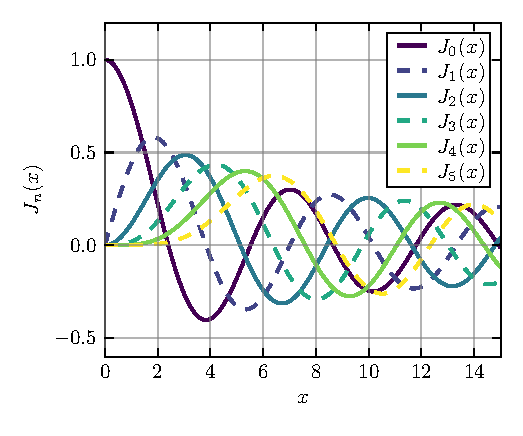
\includegraphics[width=5cm]{./plots/bessel.pdf}}
\section{Plots}
\label{sec:plots}

\begin{frame}
  \frametitle{Plotting is fun!}

  On the following pages, we include two examples on how to include plots:
  \begin{enumerate}
    \item A PDF plot
    \item A PGF/TikZ plot
  \end{enumerate}

  PDF plots are nice, but nothing beats the native look of PGF/TikZ. The source
  code to generate both plots can be found in \texttt{extra/plot\_bessel.py}
\end{frame}

\begin{frame}
  \frametitle{A Plot}
  \begin{center}
    %% Creator: Matplotlib, PGF backend
%%
%% To include the figure in your LaTeX document, write
%%   \input{<filename>.pgf}
%%
%% Make sure the required packages are loaded in your preamble
%%   \usepackage{pgf}
%%
%% Figures using additional raster images can only be included by \input if
%% they are in the same directory as the main LaTeX file. For loading figures
%% from other directories you can use the `import` package
%%   \usepackage{import}
%% and then include the figures with
%%   \import{<path to file>}{<filename>.pgf}
%%
%% Matplotlib used the following preamble
%%   \usepackage[utf8x]{inputenc}
%%   \usepackage[T1]{fontenc}
%%
\begingroup%
\makeatletter%
\begin{pgfpicture}%
\pgfpathrectangle{\pgfpointorigin}{\pgfqpoint{3.486924in}{2.905770in}}%
\pgfusepath{use as bounding box, clip}%
\begin{pgfscope}%
\pgfsetbuttcap%
\pgfsetmiterjoin%
\definecolor{currentfill}{rgb}{1.000000,1.000000,1.000000}%
\pgfsetfillcolor{currentfill}%
\pgfsetlinewidth{0.000000pt}%
\definecolor{currentstroke}{rgb}{1.000000,1.000000,1.000000}%
\pgfsetstrokecolor{currentstroke}%
\pgfsetdash{}{0pt}%
\pgfpathmoveto{\pgfqpoint{0.000000in}{0.000000in}}%
\pgfpathlineto{\pgfqpoint{3.486924in}{0.000000in}}%
\pgfpathlineto{\pgfqpoint{3.486924in}{2.905770in}}%
\pgfpathlineto{\pgfqpoint{0.000000in}{2.905770in}}%
\pgfpathclose%
\pgfusepath{fill}%
\end{pgfscope}%
\begin{pgfscope}%
\pgfsetbuttcap%
\pgfsetmiterjoin%
\definecolor{currentfill}{rgb}{1.000000,1.000000,1.000000}%
\pgfsetfillcolor{currentfill}%
\pgfsetlinewidth{0.000000pt}%
\definecolor{currentstroke}{rgb}{0.000000,0.000000,0.000000}%
\pgfsetstrokecolor{currentstroke}%
\pgfsetstrokeopacity{0.000000}%
\pgfsetdash{}{0pt}%
\pgfpathmoveto{\pgfqpoint{0.699384in}{0.529568in}}%
\pgfpathlineto{\pgfqpoint{3.336924in}{0.529568in}}%
\pgfpathlineto{\pgfqpoint{3.336924in}{2.755770in}}%
\pgfpathlineto{\pgfqpoint{0.699384in}{2.755770in}}%
\pgfpathclose%
\pgfusepath{fill}%
\end{pgfscope}%
\begin{pgfscope}%
\pgfpathrectangle{\pgfqpoint{0.699384in}{0.529568in}}{\pgfqpoint{2.637540in}{2.226203in}} %
\pgfusepath{clip}%
\pgfsetbuttcap%
\pgfsetmiterjoin%
\pgfsetlinewidth{1.505625pt}%
\definecolor{currentstroke}{rgb}{0.267004,0.004874,0.329415}%
\pgfsetstrokecolor{currentstroke}%
\pgfsetdash{}{0pt}%
\pgfpathmoveto{\pgfqpoint{0.699384in}{2.508414in}}%
\pgfpathlineto{\pgfqpoint{0.709935in}{2.507301in}}%
\pgfpathlineto{\pgfqpoint{0.720486in}{2.503965in}}%
\pgfpathlineto{\pgfqpoint{0.731565in}{2.498079in}}%
\pgfpathlineto{\pgfqpoint{0.743171in}{2.489314in}}%
\pgfpathlineto{\pgfqpoint{0.755569in}{2.477046in}}%
\pgfpathlineto{\pgfqpoint{0.768758in}{2.460751in}}%
\pgfpathlineto{\pgfqpoint{0.783002in}{2.439473in}}%
\pgfpathlineto{\pgfqpoint{0.798301in}{2.412482in}}%
\pgfpathlineto{\pgfqpoint{0.814919in}{2.378483in}}%
\pgfpathlineto{\pgfqpoint{0.832857in}{2.336571in}}%
\pgfpathlineto{\pgfqpoint{0.852376in}{2.285183in}}%
\pgfpathlineto{\pgfqpoint{0.874006in}{2.221762in}}%
\pgfpathlineto{\pgfqpoint{0.898010in}{2.144246in}}%
\pgfpathlineto{\pgfqpoint{0.925180in}{2.048757in}}%
\pgfpathlineto{\pgfqpoint{0.957625in}{1.926200in}}%
\pgfpathlineto{\pgfqpoint{1.000885in}{1.753363in}}%
\pgfpathlineto{\pgfqpoint{1.099011in}{1.358616in}}%
\pgfpathlineto{\pgfqpoint{1.132775in}{1.233656in}}%
\pgfpathlineto{\pgfqpoint{1.161263in}{1.136449in}}%
\pgfpathlineto{\pgfqpoint{1.186322in}{1.058546in}}%
\pgfpathlineto{\pgfqpoint{1.209007in}{0.995006in}}%
\pgfpathlineto{\pgfqpoint{1.229846in}{0.943028in}}%
\pgfpathlineto{\pgfqpoint{1.249102in}{0.900790in}}%
\pgfpathlineto{\pgfqpoint{1.267039in}{0.866678in}}%
\pgfpathlineto{\pgfqpoint{1.283657in}{0.839718in}}%
\pgfpathlineto{\pgfqpoint{1.299220in}{0.818601in}}%
\pgfpathlineto{\pgfqpoint{1.313728in}{0.802556in}}%
\pgfpathlineto{\pgfqpoint{1.327445in}{0.790631in}}%
\pgfpathlineto{\pgfqpoint{1.340370in}{0.782279in}}%
\pgfpathlineto{\pgfqpoint{1.352768in}{0.776883in}}%
\pgfpathlineto{\pgfqpoint{1.364638in}{0.774095in}}%
\pgfpathlineto{\pgfqpoint{1.376508in}{0.773602in}}%
\pgfpathlineto{\pgfqpoint{1.388378in}{0.775367in}}%
\pgfpathlineto{\pgfqpoint{1.400512in}{0.779457in}}%
\pgfpathlineto{\pgfqpoint{1.413173in}{0.786124in}}%
\pgfpathlineto{\pgfqpoint{1.426626in}{0.795812in}}%
\pgfpathlineto{\pgfqpoint{1.440870in}{0.808879in}}%
\pgfpathlineto{\pgfqpoint{1.456170in}{0.825983in}}%
\pgfpathlineto{\pgfqpoint{1.473052in}{0.848324in}}%
\pgfpathlineto{\pgfqpoint{1.491516in}{0.876613in}}%
\pgfpathlineto{\pgfqpoint{1.511827in}{0.911932in}}%
\pgfpathlineto{\pgfqpoint{1.534776in}{0.956456in}}%
\pgfpathlineto{\pgfqpoint{1.561418in}{1.013205in}}%
\pgfpathlineto{\pgfqpoint{1.594391in}{1.088964in}}%
\pgfpathlineto{\pgfqpoint{1.650576in}{1.224741in}}%
\pgfpathlineto{\pgfqpoint{1.701222in}{1.344768in}}%
\pgfpathlineto{\pgfqpoint{1.733403in}{1.415438in}}%
\pgfpathlineto{\pgfqpoint{1.760308in}{1.469310in}}%
\pgfpathlineto{\pgfqpoint{1.783785in}{1.511521in}}%
\pgfpathlineto{\pgfqpoint{1.805151in}{1.545494in}}%
\pgfpathlineto{\pgfqpoint{1.824671in}{1.572476in}}%
\pgfpathlineto{\pgfqpoint{1.842608in}{1.593628in}}%
\pgfpathlineto{\pgfqpoint{1.859490in}{1.610203in}}%
\pgfpathlineto{\pgfqpoint{1.875317in}{1.622715in}}%
\pgfpathlineto{\pgfqpoint{1.890352in}{1.631831in}}%
\pgfpathlineto{\pgfqpoint{1.904596in}{1.637950in}}%
\pgfpathlineto{\pgfqpoint{1.918577in}{1.641563in}}%
\pgfpathlineto{\pgfqpoint{1.932293in}{1.642809in}}%
\pgfpathlineto{\pgfqpoint{1.946010in}{1.641796in}}%
\pgfpathlineto{\pgfqpoint{1.959726in}{1.638556in}}%
\pgfpathlineto{\pgfqpoint{1.973971in}{1.632879in}}%
\pgfpathlineto{\pgfqpoint{1.988742in}{1.624570in}}%
\pgfpathlineto{\pgfqpoint{2.004305in}{1.613244in}}%
\pgfpathlineto{\pgfqpoint{2.020924in}{1.598366in}}%
\pgfpathlineto{\pgfqpoint{2.038861in}{1.579269in}}%
\pgfpathlineto{\pgfqpoint{2.058380in}{1.555174in}}%
\pgfpathlineto{\pgfqpoint{2.080010in}{1.524843in}}%
\pgfpathlineto{\pgfqpoint{2.104542in}{1.486447in}}%
\pgfpathlineto{\pgfqpoint{2.133030in}{1.437557in}}%
\pgfpathlineto{\pgfqpoint{2.169696in}{1.369912in}}%
\pgfpathlineto{\pgfqpoint{2.281275in}{1.161006in}}%
\pgfpathlineto{\pgfqpoint{2.310554in}{1.112613in}}%
\pgfpathlineto{\pgfqpoint{2.335877in}{1.074938in}}%
\pgfpathlineto{\pgfqpoint{2.358562in}{1.045091in}}%
\pgfpathlineto{\pgfqpoint{2.379137in}{1.021596in}}%
\pgfpathlineto{\pgfqpoint{2.398130in}{1.003173in}}%
\pgfpathlineto{\pgfqpoint{2.416067in}{0.988816in}}%
\pgfpathlineto{\pgfqpoint{2.432949in}{0.978111in}}%
\pgfpathlineto{\pgfqpoint{2.449039in}{0.970507in}}%
\pgfpathlineto{\pgfqpoint{2.464602in}{0.965605in}}%
\pgfpathlineto{\pgfqpoint{2.479638in}{0.963176in}}%
\pgfpathlineto{\pgfqpoint{2.494673in}{0.963011in}}%
\pgfpathlineto{\pgfqpoint{2.509709in}{0.965094in}}%
\pgfpathlineto{\pgfqpoint{2.525008in}{0.969485in}}%
\pgfpathlineto{\pgfqpoint{2.540835in}{0.976383in}}%
\pgfpathlineto{\pgfqpoint{2.557453in}{0.986124in}}%
\pgfpathlineto{\pgfqpoint{2.574862in}{0.998953in}}%
\pgfpathlineto{\pgfqpoint{2.593591in}{1.015586in}}%
\pgfpathlineto{\pgfqpoint{2.613902in}{1.036697in}}%
\pgfpathlineto{\pgfqpoint{2.636059in}{1.063013in}}%
\pgfpathlineto{\pgfqpoint{2.661119in}{1.096352in}}%
\pgfpathlineto{\pgfqpoint{2.690398in}{1.139191in}}%
\pgfpathlineto{\pgfqpoint{2.727855in}{1.198210in}}%
\pgfpathlineto{\pgfqpoint{2.837851in}{1.374049in}}%
\pgfpathlineto{\pgfqpoint{2.867659in}{1.416094in}}%
\pgfpathlineto{\pgfqpoint{2.893245in}{1.448486in}}%
\pgfpathlineto{\pgfqpoint{2.916194in}{1.474074in}}%
\pgfpathlineto{\pgfqpoint{2.937297in}{1.494356in}}%
\pgfpathlineto{\pgfqpoint{2.956816in}{1.510113in}}%
\pgfpathlineto{\pgfqpoint{2.975281in}{1.522205in}}%
\pgfpathlineto{\pgfqpoint{2.992691in}{1.531000in}}%
\pgfpathlineto{\pgfqpoint{3.009309in}{1.536973in}}%
\pgfpathlineto{\pgfqpoint{3.025663in}{1.540506in}}%
\pgfpathlineto{\pgfqpoint{3.041754in}{1.541697in}}%
\pgfpathlineto{\pgfqpoint{3.057844in}{1.540627in}}%
\pgfpathlineto{\pgfqpoint{3.073935in}{1.537322in}}%
\pgfpathlineto{\pgfqpoint{3.090553in}{1.531606in}}%
\pgfpathlineto{\pgfqpoint{3.107699in}{1.523328in}}%
\pgfpathlineto{\pgfqpoint{3.125900in}{1.512000in}}%
\pgfpathlineto{\pgfqpoint{3.145156in}{1.497320in}}%
\pgfpathlineto{\pgfqpoint{3.165731in}{1.478791in}}%
\pgfpathlineto{\pgfqpoint{3.188416in}{1.455281in}}%
\pgfpathlineto{\pgfqpoint{3.213739in}{1.425722in}}%
\pgfpathlineto{\pgfqpoint{3.243018in}{1.388000in}}%
\pgfpathlineto{\pgfqpoint{3.280475in}{1.335861in}}%
\pgfpathlineto{\pgfqpoint{3.336924in}{1.254042in}}%
\pgfpathlineto{\pgfqpoint{3.336924in}{1.254042in}}%
\pgfusepath{stroke}%
\end{pgfscope}%
\begin{pgfscope}%
\pgfpathrectangle{\pgfqpoint{0.699384in}{0.529568in}}{\pgfqpoint{2.637540in}{2.226203in}} %
\pgfusepath{clip}%
\pgfsetbuttcap%
\pgfsetmiterjoin%
\pgfsetlinewidth{1.505625pt}%
\definecolor{currentstroke}{rgb}{0.253935,0.265254,0.529983}%
\pgfsetstrokecolor{currentstroke}%
\pgfsetdash{{6.000000pt}{6.000000pt}}{0.000000pt}%
\pgfpathmoveto{\pgfqpoint{0.699384in}{1.271635in}}%
\pgfpathlineto{\pgfqpoint{0.765329in}{1.499501in}}%
\pgfpathlineto{\pgfqpoint{0.799884in}{1.610842in}}%
\pgfpathlineto{\pgfqpoint{0.828372in}{1.695431in}}%
\pgfpathlineto{\pgfqpoint{0.853168in}{1.762382in}}%
\pgfpathlineto{\pgfqpoint{0.875589in}{1.816724in}}%
\pgfpathlineto{\pgfqpoint{0.895900in}{1.860321in}}%
\pgfpathlineto{\pgfqpoint{0.914628in}{1.895411in}}%
\pgfpathlineto{\pgfqpoint{0.931774in}{1.922998in}}%
\pgfpathlineto{\pgfqpoint{0.947865in}{1.944784in}}%
\pgfpathlineto{\pgfqpoint{0.962636in}{1.961184in}}%
\pgfpathlineto{\pgfqpoint{0.976617in}{1.973468in}}%
\pgfpathlineto{\pgfqpoint{0.989806in}{1.982134in}}%
\pgfpathlineto{\pgfqpoint{1.002204in}{1.987672in}}%
\pgfpathlineto{\pgfqpoint{1.014074in}{1.990600in}}%
\pgfpathlineto{\pgfqpoint{1.025680in}{1.991220in}}%
\pgfpathlineto{\pgfqpoint{1.037286in}{1.989634in}}%
\pgfpathlineto{\pgfqpoint{1.049156in}{1.985749in}}%
\pgfpathlineto{\pgfqpoint{1.061554in}{1.979277in}}%
\pgfpathlineto{\pgfqpoint{1.074479in}{1.969949in}}%
\pgfpathlineto{\pgfqpoint{1.088196in}{1.957234in}}%
\pgfpathlineto{\pgfqpoint{1.102968in}{1.940390in}}%
\pgfpathlineto{\pgfqpoint{1.118794in}{1.918855in}}%
\pgfpathlineto{\pgfqpoint{1.135940in}{1.891647in}}%
\pgfpathlineto{\pgfqpoint{1.154669in}{1.857604in}}%
\pgfpathlineto{\pgfqpoint{1.175243in}{1.815419in}}%
\pgfpathlineto{\pgfqpoint{1.198192in}{1.763083in}}%
\pgfpathlineto{\pgfqpoint{1.224307in}{1.697736in}}%
\pgfpathlineto{\pgfqpoint{1.255169in}{1.614225in}}%
\pgfpathlineto{\pgfqpoint{1.296582in}{1.495185in}}%
\pgfpathlineto{\pgfqpoint{1.391016in}{1.221723in}}%
\pgfpathlineto{\pgfqpoint{1.423197in}{1.136562in}}%
\pgfpathlineto{\pgfqpoint{1.450366in}{1.070703in}}%
\pgfpathlineto{\pgfqpoint{1.474370in}{1.018130in}}%
\pgfpathlineto{\pgfqpoint{1.496000in}{0.975887in}}%
\pgfpathlineto{\pgfqpoint{1.516048in}{0.941483in}}%
\pgfpathlineto{\pgfqpoint{1.534512in}{0.914101in}}%
\pgfpathlineto{\pgfqpoint{1.551658in}{0.892542in}}%
\pgfpathlineto{\pgfqpoint{1.567749in}{0.875804in}}%
\pgfpathlineto{\pgfqpoint{1.582784in}{0.863285in}}%
\pgfpathlineto{\pgfqpoint{1.597028in}{0.854241in}}%
\pgfpathlineto{\pgfqpoint{1.610745in}{0.848135in}}%
\pgfpathlineto{\pgfqpoint{1.623934in}{0.844671in}}%
\pgfpathlineto{\pgfqpoint{1.636859in}{0.843553in}}%
\pgfpathlineto{\pgfqpoint{1.649784in}{0.844667in}}%
\pgfpathlineto{\pgfqpoint{1.662973in}{0.848067in}}%
\pgfpathlineto{\pgfqpoint{1.676426in}{0.853844in}}%
\pgfpathlineto{\pgfqpoint{1.690670in}{0.862433in}}%
\pgfpathlineto{\pgfqpoint{1.705706in}{0.874165in}}%
\pgfpathlineto{\pgfqpoint{1.721797in}{0.889619in}}%
\pgfpathlineto{\pgfqpoint{1.739206in}{0.909530in}}%
\pgfpathlineto{\pgfqpoint{1.758198in}{0.934763in}}%
\pgfpathlineto{\pgfqpoint{1.779037in}{0.966272in}}%
\pgfpathlineto{\pgfqpoint{1.802513in}{1.005971in}}%
\pgfpathlineto{\pgfqpoint{1.829419in}{1.056000in}}%
\pgfpathlineto{\pgfqpoint{1.862655in}{1.122749in}}%
\pgfpathlineto{\pgfqpoint{1.917258in}{1.238284in}}%
\pgfpathlineto{\pgfqpoint{1.970541in}{1.349167in}}%
\pgfpathlineto{\pgfqpoint{2.003250in}{1.412169in}}%
\pgfpathlineto{\pgfqpoint{2.030420in}{1.459815in}}%
\pgfpathlineto{\pgfqpoint{2.054160in}{1.497121in}}%
\pgfpathlineto{\pgfqpoint{2.075790in}{1.527077in}}%
\pgfpathlineto{\pgfqpoint{2.095573in}{1.550775in}}%
\pgfpathlineto{\pgfqpoint{2.114038in}{1.569485in}}%
\pgfpathlineto{\pgfqpoint{2.131184in}{1.583770in}}%
\pgfpathlineto{\pgfqpoint{2.147274in}{1.594381in}}%
\pgfpathlineto{\pgfqpoint{2.162837in}{1.602016in}}%
\pgfpathlineto{\pgfqpoint{2.177609in}{1.606842in}}%
\pgfpathlineto{\pgfqpoint{2.192117in}{1.609278in}}%
\pgfpathlineto{\pgfqpoint{2.206361in}{1.609454in}}%
\pgfpathlineto{\pgfqpoint{2.220869in}{1.607395in}}%
\pgfpathlineto{\pgfqpoint{2.235641in}{1.603014in}}%
\pgfpathlineto{\pgfqpoint{2.250940in}{1.596102in}}%
\pgfpathlineto{\pgfqpoint{2.266767in}{1.586486in}}%
\pgfpathlineto{\pgfqpoint{2.283649in}{1.573578in}}%
\pgfpathlineto{\pgfqpoint{2.301850in}{1.556758in}}%
\pgfpathlineto{\pgfqpoint{2.321369in}{1.535605in}}%
\pgfpathlineto{\pgfqpoint{2.342736in}{1.509093in}}%
\pgfpathlineto{\pgfqpoint{2.366740in}{1.475635in}}%
\pgfpathlineto{\pgfqpoint{2.394437in}{1.433039in}}%
\pgfpathlineto{\pgfqpoint{2.428728in}{1.375949in}}%
\pgfpathlineto{\pgfqpoint{2.489134in}{1.270076in}}%
\pgfpathlineto{\pgfqpoint{2.537669in}{1.187120in}}%
\pgfpathlineto{\pgfqpoint{2.569851in}{1.136413in}}%
\pgfpathlineto{\pgfqpoint{2.596756in}{1.098029in}}%
\pgfpathlineto{\pgfqpoint{2.620496in}{1.067902in}}%
\pgfpathlineto{\pgfqpoint{2.642126in}{1.043946in}}%
\pgfpathlineto{\pgfqpoint{2.662174in}{1.025004in}}%
\pgfpathlineto{\pgfqpoint{2.680638in}{1.010519in}}%
\pgfpathlineto{\pgfqpoint{2.698048in}{0.999586in}}%
\pgfpathlineto{\pgfqpoint{2.714666in}{0.991693in}}%
\pgfpathlineto{\pgfqpoint{2.730757in}{0.986465in}}%
\pgfpathlineto{\pgfqpoint{2.746583in}{0.983664in}}%
\pgfpathlineto{\pgfqpoint{2.762146in}{0.983180in}}%
\pgfpathlineto{\pgfqpoint{2.777710in}{0.984932in}}%
\pgfpathlineto{\pgfqpoint{2.793536in}{0.988977in}}%
\pgfpathlineto{\pgfqpoint{2.809891in}{0.995503in}}%
\pgfpathlineto{\pgfqpoint{2.826773in}{1.004662in}}%
\pgfpathlineto{\pgfqpoint{2.844710in}{1.016977in}}%
\pgfpathlineto{\pgfqpoint{2.863702in}{1.032755in}}%
\pgfpathlineto{\pgfqpoint{2.884277in}{1.052794in}}%
\pgfpathlineto{\pgfqpoint{2.906962in}{1.078087in}}%
\pgfpathlineto{\pgfqpoint{2.932285in}{1.109750in}}%
\pgfpathlineto{\pgfqpoint{2.962092in}{1.150752in}}%
\pgfpathlineto{\pgfqpoint{3.000340in}{1.207417in}}%
\pgfpathlineto{\pgfqpoint{3.107699in}{1.368630in}}%
\pgfpathlineto{\pgfqpoint{3.138034in}{1.408933in}}%
\pgfpathlineto{\pgfqpoint{3.164148in}{1.440040in}}%
\pgfpathlineto{\pgfqpoint{3.187361in}{1.464353in}}%
\pgfpathlineto{\pgfqpoint{3.208727in}{1.483605in}}%
\pgfpathlineto{\pgfqpoint{3.228510in}{1.498528in}}%
\pgfpathlineto{\pgfqpoint{3.247239in}{1.509930in}}%
\pgfpathlineto{\pgfqpoint{3.264912in}{1.518158in}}%
\pgfpathlineto{\pgfqpoint{3.282058in}{1.523728in}}%
\pgfpathlineto{\pgfqpoint{3.298676in}{1.526825in}}%
\pgfpathlineto{\pgfqpoint{3.315030in}{1.527646in}}%
\pgfpathlineto{\pgfqpoint{3.331385in}{1.526266in}}%
\pgfpathlineto{\pgfqpoint{3.336924in}{1.525303in}}%
\pgfpathlineto{\pgfqpoint{3.336924in}{1.525303in}}%
\pgfusepath{stroke}%
\end{pgfscope}%
\begin{pgfscope}%
\pgfpathrectangle{\pgfqpoint{0.699384in}{0.529568in}}{\pgfqpoint{2.637540in}{2.226203in}} %
\pgfusepath{clip}%
\pgfsetbuttcap%
\pgfsetmiterjoin%
\pgfsetlinewidth{1.505625pt}%
\definecolor{currentstroke}{rgb}{0.163625,0.471133,0.558148}%
\pgfsetstrokecolor{currentstroke}%
\pgfsetdash{}{0pt}%
\pgfpathmoveto{\pgfqpoint{0.699384in}{1.271635in}}%
\pgfpathlineto{\pgfqpoint{0.714419in}{1.272765in}}%
\pgfpathlineto{\pgfqpoint{0.729455in}{1.276145in}}%
\pgfpathlineto{\pgfqpoint{0.744754in}{1.281871in}}%
\pgfpathlineto{\pgfqpoint{0.760581in}{1.290173in}}%
\pgfpathlineto{\pgfqpoint{0.777199in}{1.301421in}}%
\pgfpathlineto{\pgfqpoint{0.794872in}{1.316117in}}%
\pgfpathlineto{\pgfqpoint{0.813864in}{1.334882in}}%
\pgfpathlineto{\pgfqpoint{0.834439in}{1.358437in}}%
\pgfpathlineto{\pgfqpoint{0.857124in}{1.387914in}}%
\pgfpathlineto{\pgfqpoint{0.882711in}{1.424971in}}%
\pgfpathlineto{\pgfqpoint{0.912782in}{1.472645in}}%
\pgfpathlineto{\pgfqpoint{0.952613in}{1.540325in}}%
\pgfpathlineto{\pgfqpoint{1.042562in}{1.694481in}}%
\pgfpathlineto{\pgfqpoint{1.072897in}{1.741246in}}%
\pgfpathlineto{\pgfqpoint{1.098220in}{1.776374in}}%
\pgfpathlineto{\pgfqpoint{1.120641in}{1.803811in}}%
\pgfpathlineto{\pgfqpoint{1.140952in}{1.825246in}}%
\pgfpathlineto{\pgfqpoint{1.159417in}{1.841613in}}%
\pgfpathlineto{\pgfqpoint{1.176562in}{1.853947in}}%
\pgfpathlineto{\pgfqpoint{1.192653in}{1.862869in}}%
\pgfpathlineto{\pgfqpoint{1.207952in}{1.868868in}}%
\pgfpathlineto{\pgfqpoint{1.222724in}{1.872288in}}%
\pgfpathlineto{\pgfqpoint{1.236968in}{1.873325in}}%
\pgfpathlineto{\pgfqpoint{1.250948in}{1.872150in}}%
\pgfpathlineto{\pgfqpoint{1.265193in}{1.868696in}}%
\pgfpathlineto{\pgfqpoint{1.279701in}{1.862826in}}%
\pgfpathlineto{\pgfqpoint{1.294472in}{1.854416in}}%
\pgfpathlineto{\pgfqpoint{1.310035in}{1.842921in}}%
\pgfpathlineto{\pgfqpoint{1.326390in}{1.827973in}}%
\pgfpathlineto{\pgfqpoint{1.343535in}{1.809222in}}%
\pgfpathlineto{\pgfqpoint{1.362000in}{1.785627in}}%
\pgfpathlineto{\pgfqpoint{1.381784in}{1.756619in}}%
\pgfpathlineto{\pgfqpoint{1.403150in}{1.721244in}}%
\pgfpathlineto{\pgfqpoint{1.426626in}{1.677960in}}%
\pgfpathlineto{\pgfqpoint{1.453004in}{1.624491in}}%
\pgfpathlineto{\pgfqpoint{1.483603in}{1.557204in}}%
\pgfpathlineto{\pgfqpoint{1.522115in}{1.466772in}}%
\pgfpathlineto{\pgfqpoint{1.649784in}{1.162461in}}%
\pgfpathlineto{\pgfqpoint{1.679855in}{1.099015in}}%
\pgfpathlineto{\pgfqpoint{1.705970in}{1.048936in}}%
\pgfpathlineto{\pgfqpoint{1.729182in}{1.009044in}}%
\pgfpathlineto{\pgfqpoint{1.750549in}{0.976630in}}%
\pgfpathlineto{\pgfqpoint{1.770068in}{0.950923in}}%
\pgfpathlineto{\pgfqpoint{1.788269in}{0.930514in}}%
\pgfpathlineto{\pgfqpoint{1.805415in}{0.914562in}}%
\pgfpathlineto{\pgfqpoint{1.821506in}{0.902566in}}%
\pgfpathlineto{\pgfqpoint{1.836805in}{0.893884in}}%
\pgfpathlineto{\pgfqpoint{1.851576in}{0.888046in}}%
\pgfpathlineto{\pgfqpoint{1.865821in}{0.884797in}}%
\pgfpathlineto{\pgfqpoint{1.879801in}{0.883876in}}%
\pgfpathlineto{\pgfqpoint{1.893781in}{0.885185in}}%
\pgfpathlineto{\pgfqpoint{1.908025in}{0.888783in}}%
\pgfpathlineto{\pgfqpoint{1.922533in}{0.894753in}}%
\pgfpathlineto{\pgfqpoint{1.937833in}{0.903504in}}%
\pgfpathlineto{\pgfqpoint{1.953923in}{0.915336in}}%
\pgfpathlineto{\pgfqpoint{1.971069in}{0.930780in}}%
\pgfpathlineto{\pgfqpoint{1.989534in}{0.950497in}}%
\pgfpathlineto{\pgfqpoint{2.009581in}{0.975260in}}%
\pgfpathlineto{\pgfqpoint{2.031739in}{1.006302in}}%
\pgfpathlineto{\pgfqpoint{2.056534in}{1.045010in}}%
\pgfpathlineto{\pgfqpoint{2.085286in}{1.094171in}}%
\pgfpathlineto{\pgfqpoint{2.121688in}{1.161084in}}%
\pgfpathlineto{\pgfqpoint{2.244346in}{1.390303in}}%
\pgfpathlineto{\pgfqpoint{2.273361in}{1.437736in}}%
\pgfpathlineto{\pgfqpoint{2.298684in}{1.474987in}}%
\pgfpathlineto{\pgfqpoint{2.321369in}{1.504503in}}%
\pgfpathlineto{\pgfqpoint{2.342208in}{1.528035in}}%
\pgfpathlineto{\pgfqpoint{2.361464in}{1.546489in}}%
\pgfpathlineto{\pgfqpoint{2.379401in}{1.560677in}}%
\pgfpathlineto{\pgfqpoint{2.396283in}{1.571284in}}%
\pgfpathlineto{\pgfqpoint{2.412374in}{1.578850in}}%
\pgfpathlineto{\pgfqpoint{2.427937in}{1.583769in}}%
\pgfpathlineto{\pgfqpoint{2.443236in}{1.586288in}}%
\pgfpathlineto{\pgfqpoint{2.458271in}{1.586527in}}%
\pgfpathlineto{\pgfqpoint{2.473307in}{1.584565in}}%
\pgfpathlineto{\pgfqpoint{2.488606in}{1.580340in}}%
\pgfpathlineto{\pgfqpoint{2.504433in}{1.573655in}}%
\pgfpathlineto{\pgfqpoint{2.521051in}{1.564179in}}%
\pgfpathlineto{\pgfqpoint{2.538461in}{1.551662in}}%
\pgfpathlineto{\pgfqpoint{2.557189in}{1.535396in}}%
\pgfpathlineto{\pgfqpoint{2.577500in}{1.514706in}}%
\pgfpathlineto{\pgfqpoint{2.599658in}{1.488853in}}%
\pgfpathlineto{\pgfqpoint{2.624453in}{1.456379in}}%
\pgfpathlineto{\pgfqpoint{2.653205in}{1.414878in}}%
\pgfpathlineto{\pgfqpoint{2.689079in}{1.358935in}}%
\pgfpathlineto{\pgfqpoint{2.817804in}{1.154392in}}%
\pgfpathlineto{\pgfqpoint{2.846292in}{1.115386in}}%
\pgfpathlineto{\pgfqpoint{2.871352in}{1.084744in}}%
\pgfpathlineto{\pgfqpoint{2.893773in}{1.060721in}}%
\pgfpathlineto{\pgfqpoint{2.914612in}{1.041582in}}%
\pgfpathlineto{\pgfqpoint{2.933868in}{1.026836in}}%
\pgfpathlineto{\pgfqpoint{2.952068in}{1.015630in}}%
\pgfpathlineto{\pgfqpoint{2.969478in}{1.007487in}}%
\pgfpathlineto{\pgfqpoint{2.986096in}{1.002118in}}%
\pgfpathlineto{\pgfqpoint{3.002450in}{0.999157in}}%
\pgfpathlineto{\pgfqpoint{3.018541in}{0.998501in}}%
\pgfpathlineto{\pgfqpoint{3.034632in}{1.000075in}}%
\pgfpathlineto{\pgfqpoint{3.050986in}{1.003932in}}%
\pgfpathlineto{\pgfqpoint{3.067868in}{1.010250in}}%
\pgfpathlineto{\pgfqpoint{3.085278in}{1.019174in}}%
\pgfpathlineto{\pgfqpoint{3.103742in}{1.031199in}}%
\pgfpathlineto{\pgfqpoint{3.123262in}{1.046616in}}%
\pgfpathlineto{\pgfqpoint{3.144364in}{1.066176in}}%
\pgfpathlineto{\pgfqpoint{3.167577in}{1.090813in}}%
\pgfpathlineto{\pgfqpoint{3.193691in}{1.121898in}}%
\pgfpathlineto{\pgfqpoint{3.224290in}{1.161945in}}%
\pgfpathlineto{\pgfqpoint{3.264384in}{1.218378in}}%
\pgfpathlineto{\pgfqpoint{3.336924in}{1.323050in}}%
\pgfpathlineto{\pgfqpoint{3.336924in}{1.323050in}}%
\pgfusepath{stroke}%
\end{pgfscope}%
\begin{pgfscope}%
\pgfpathrectangle{\pgfqpoint{0.699384in}{0.529568in}}{\pgfqpoint{2.637540in}{2.226203in}} %
\pgfusepath{clip}%
\pgfsetbuttcap%
\pgfsetmiterjoin%
\pgfsetlinewidth{1.505625pt}%
\definecolor{currentstroke}{rgb}{0.134692,0.658636,0.517649}%
\pgfsetstrokecolor{currentstroke}%
\pgfsetdash{{6.000000pt}{6.000000pt}}{0.000000pt}%
\pgfpathmoveto{\pgfqpoint{0.699384in}{1.271635in}}%
\pgfpathlineto{\pgfqpoint{0.761108in}{1.272741in}}%
\pgfpathlineto{\pgfqpoint{0.794345in}{1.275620in}}%
\pgfpathlineto{\pgfqpoint{0.822833in}{1.280280in}}%
\pgfpathlineto{\pgfqpoint{0.848947in}{1.286787in}}%
\pgfpathlineto{\pgfqpoint{0.873742in}{1.295251in}}%
\pgfpathlineto{\pgfqpoint{0.898010in}{1.305906in}}%
\pgfpathlineto{\pgfqpoint{0.922014in}{1.318898in}}%
\pgfpathlineto{\pgfqpoint{0.946282in}{1.334598in}}%
\pgfpathlineto{\pgfqpoint{0.971077in}{1.353324in}}%
\pgfpathlineto{\pgfqpoint{0.996928in}{1.375677in}}%
\pgfpathlineto{\pgfqpoint{1.024361in}{1.402400in}}%
\pgfpathlineto{\pgfqpoint{1.054168in}{1.434615in}}%
\pgfpathlineto{\pgfqpoint{1.087932in}{1.474488in}}%
\pgfpathlineto{\pgfqpoint{1.130137in}{1.527989in}}%
\pgfpathlineto{\pgfqpoint{1.248838in}{1.680569in}}%
\pgfpathlineto{\pgfqpoint{1.279964in}{1.715696in}}%
\pgfpathlineto{\pgfqpoint{1.306342in}{1.742218in}}%
\pgfpathlineto{\pgfqpoint{1.329819in}{1.762759in}}%
\pgfpathlineto{\pgfqpoint{1.351185in}{1.778571in}}%
\pgfpathlineto{\pgfqpoint{1.370969in}{1.790499in}}%
\pgfpathlineto{\pgfqpoint{1.389433in}{1.799088in}}%
\pgfpathlineto{\pgfqpoint{1.406843in}{1.804796in}}%
\pgfpathlineto{\pgfqpoint{1.423725in}{1.808011in}}%
\pgfpathlineto{\pgfqpoint{1.440079in}{1.808868in}}%
\pgfpathlineto{\pgfqpoint{1.456170in}{1.807484in}}%
\pgfpathlineto{\pgfqpoint{1.472260in}{1.803847in}}%
\pgfpathlineto{\pgfqpoint{1.488351in}{1.797931in}}%
\pgfpathlineto{\pgfqpoint{1.504969in}{1.789414in}}%
\pgfpathlineto{\pgfqpoint{1.522115in}{1.778071in}}%
\pgfpathlineto{\pgfqpoint{1.540052in}{1.763454in}}%
\pgfpathlineto{\pgfqpoint{1.558780in}{1.745248in}}%
\pgfpathlineto{\pgfqpoint{1.578564in}{1.722851in}}%
\pgfpathlineto{\pgfqpoint{1.599666in}{1.695533in}}%
\pgfpathlineto{\pgfqpoint{1.622351in}{1.662465in}}%
\pgfpathlineto{\pgfqpoint{1.647147in}{1.622309in}}%
\pgfpathlineto{\pgfqpoint{1.674844in}{1.573097in}}%
\pgfpathlineto{\pgfqpoint{1.706761in}{1.511693in}}%
\pgfpathlineto{\pgfqpoint{1.747119in}{1.428912in}}%
\pgfpathlineto{\pgfqpoint{1.875317in}{1.162218in}}%
\pgfpathlineto{\pgfqpoint{1.906443in}{1.104664in}}%
\pgfpathlineto{\pgfqpoint{1.933348in}{1.059412in}}%
\pgfpathlineto{\pgfqpoint{1.957352in}{1.023229in}}%
\pgfpathlineto{\pgfqpoint{1.979246in}{0.994104in}}%
\pgfpathlineto{\pgfqpoint{1.999557in}{0.970684in}}%
\pgfpathlineto{\pgfqpoint{2.018549in}{0.952118in}}%
\pgfpathlineto{\pgfqpoint{2.036223in}{0.937868in}}%
\pgfpathlineto{\pgfqpoint{2.053105in}{0.927068in}}%
\pgfpathlineto{\pgfqpoint{2.069195in}{0.919390in}}%
\pgfpathlineto{\pgfqpoint{2.084758in}{0.914423in}}%
\pgfpathlineto{\pgfqpoint{2.099794in}{0.911935in}}%
\pgfpathlineto{\pgfqpoint{2.114829in}{0.911718in}}%
\pgfpathlineto{\pgfqpoint{2.129865in}{0.913755in}}%
\pgfpathlineto{\pgfqpoint{2.145164in}{0.918114in}}%
\pgfpathlineto{\pgfqpoint{2.160991in}{0.925002in}}%
\pgfpathlineto{\pgfqpoint{2.177345in}{0.934590in}}%
\pgfpathlineto{\pgfqpoint{2.194755in}{0.947458in}}%
\pgfpathlineto{\pgfqpoint{2.213219in}{0.963960in}}%
\pgfpathlineto{\pgfqpoint{2.233003in}{0.984699in}}%
\pgfpathlineto{\pgfqpoint{2.254633in}{1.010697in}}%
\pgfpathlineto{\pgfqpoint{2.278637in}{1.043168in}}%
\pgfpathlineto{\pgfqpoint{2.305806in}{1.083821in}}%
\pgfpathlineto{\pgfqpoint{2.338251in}{1.136581in}}%
\pgfpathlineto{\pgfqpoint{2.383358in}{1.214606in}}%
\pgfpathlineto{\pgfqpoint{2.462492in}{1.351721in}}%
\pgfpathlineto{\pgfqpoint{2.495992in}{1.404951in}}%
\pgfpathlineto{\pgfqpoint{2.523953in}{1.445346in}}%
\pgfpathlineto{\pgfqpoint{2.548484in}{1.477024in}}%
\pgfpathlineto{\pgfqpoint{2.570906in}{1.502436in}}%
\pgfpathlineto{\pgfqpoint{2.591481in}{1.522479in}}%
\pgfpathlineto{\pgfqpoint{2.610737in}{1.538193in}}%
\pgfpathlineto{\pgfqpoint{2.628674in}{1.550051in}}%
\pgfpathlineto{\pgfqpoint{2.645819in}{1.558792in}}%
\pgfpathlineto{\pgfqpoint{2.662437in}{1.564789in}}%
\pgfpathlineto{\pgfqpoint{2.678528in}{1.568244in}}%
\pgfpathlineto{\pgfqpoint{2.694355in}{1.569375in}}%
\pgfpathlineto{\pgfqpoint{2.710182in}{1.568264in}}%
\pgfpathlineto{\pgfqpoint{2.726009in}{1.564933in}}%
\pgfpathlineto{\pgfqpoint{2.742363in}{1.559203in}}%
\pgfpathlineto{\pgfqpoint{2.759245in}{1.550913in}}%
\pgfpathlineto{\pgfqpoint{2.777182in}{1.539558in}}%
\pgfpathlineto{\pgfqpoint{2.796174in}{1.524816in}}%
\pgfpathlineto{\pgfqpoint{2.816485in}{1.506158in}}%
\pgfpathlineto{\pgfqpoint{2.838643in}{1.482688in}}%
\pgfpathlineto{\pgfqpoint{2.863174in}{1.453355in}}%
\pgfpathlineto{\pgfqpoint{2.891135in}{1.416332in}}%
\pgfpathlineto{\pgfqpoint{2.925163in}{1.367391in}}%
\pgfpathlineto{\pgfqpoint{2.977919in}{1.287023in}}%
\pgfpathlineto{\pgfqpoint{3.037797in}{1.196847in}}%
\pgfpathlineto{\pgfqpoint{3.071825in}{1.149633in}}%
\pgfpathlineto{\pgfqpoint{3.100049in}{1.114180in}}%
\pgfpathlineto{\pgfqpoint{3.124845in}{1.086512in}}%
\pgfpathlineto{\pgfqpoint{3.147266in}{1.064723in}}%
\pgfpathlineto{\pgfqpoint{3.168105in}{1.047503in}}%
\pgfpathlineto{\pgfqpoint{3.187624in}{1.034213in}}%
\pgfpathlineto{\pgfqpoint{3.206089in}{1.024294in}}%
\pgfpathlineto{\pgfqpoint{3.223762in}{1.017297in}}%
\pgfpathlineto{\pgfqpoint{3.240908in}{1.012894in}}%
\pgfpathlineto{\pgfqpoint{3.257526in}{1.010892in}}%
\pgfpathlineto{\pgfqpoint{3.274144in}{1.011125in}}%
\pgfpathlineto{\pgfqpoint{3.290762in}{1.013576in}}%
\pgfpathlineto{\pgfqpoint{3.307644in}{1.018303in}}%
\pgfpathlineto{\pgfqpoint{3.325318in}{1.025608in}}%
\pgfpathlineto{\pgfqpoint{3.336924in}{1.031677in}}%
\pgfpathlineto{\pgfqpoint{3.336924in}{1.031677in}}%
\pgfusepath{stroke}%
\end{pgfscope}%
\begin{pgfscope}%
\pgfpathrectangle{\pgfqpoint{0.699384in}{0.529568in}}{\pgfqpoint{2.637540in}{2.226203in}} %
\pgfusepath{clip}%
\pgfsetbuttcap%
\pgfsetmiterjoin%
\pgfsetlinewidth{1.505625pt}%
\definecolor{currentstroke}{rgb}{0.477504,0.821444,0.318195}%
\pgfsetstrokecolor{currentstroke}%
\pgfsetdash{}{0pt}%
\pgfpathmoveto{\pgfqpoint{0.699384in}{1.271635in}}%
\pgfpathlineto{\pgfqpoint{0.834967in}{1.272740in}}%
\pgfpathlineto{\pgfqpoint{0.885876in}{1.275487in}}%
\pgfpathlineto{\pgfqpoint{0.926235in}{1.279840in}}%
\pgfpathlineto{\pgfqpoint{0.961318in}{1.285814in}}%
\pgfpathlineto{\pgfqpoint{0.993499in}{1.293519in}}%
\pgfpathlineto{\pgfqpoint{1.023834in}{1.303048in}}%
\pgfpathlineto{\pgfqpoint{1.053113in}{1.314568in}}%
\pgfpathlineto{\pgfqpoint{1.081865in}{1.328273in}}%
\pgfpathlineto{\pgfqpoint{1.110617in}{1.344456in}}%
\pgfpathlineto{\pgfqpoint{1.139897in}{1.363528in}}%
\pgfpathlineto{\pgfqpoint{1.169968in}{1.385807in}}%
\pgfpathlineto{\pgfqpoint{1.201622in}{1.412068in}}%
\pgfpathlineto{\pgfqpoint{1.235913in}{1.443466in}}%
\pgfpathlineto{\pgfqpoint{1.274952in}{1.482325in}}%
\pgfpathlineto{\pgfqpoint{1.325862in}{1.536387in}}%
\pgfpathlineto{\pgfqpoint{1.425044in}{1.642301in}}%
\pgfpathlineto{\pgfqpoint{1.460918in}{1.676888in}}%
\pgfpathlineto{\pgfqpoint{1.490725in}{1.702621in}}%
\pgfpathlineto{\pgfqpoint{1.516839in}{1.722309in}}%
\pgfpathlineto{\pgfqpoint{1.540579in}{1.737477in}}%
\pgfpathlineto{\pgfqpoint{1.562473in}{1.748866in}}%
\pgfpathlineto{\pgfqpoint{1.582784in}{1.756988in}}%
\pgfpathlineto{\pgfqpoint{1.602040in}{1.762356in}}%
\pgfpathlineto{\pgfqpoint{1.620505in}{1.765252in}}%
\pgfpathlineto{\pgfqpoint{1.638442in}{1.765859in}}%
\pgfpathlineto{\pgfqpoint{1.656115in}{1.764261in}}%
\pgfpathlineto{\pgfqpoint{1.673788in}{1.760427in}}%
\pgfpathlineto{\pgfqpoint{1.691462in}{1.754319in}}%
\pgfpathlineto{\pgfqpoint{1.709663in}{1.745631in}}%
\pgfpathlineto{\pgfqpoint{1.728127in}{1.734327in}}%
\pgfpathlineto{\pgfqpoint{1.747383in}{1.719886in}}%
\pgfpathlineto{\pgfqpoint{1.767431in}{1.702024in}}%
\pgfpathlineto{\pgfqpoint{1.788533in}{1.680194in}}%
\pgfpathlineto{\pgfqpoint{1.810954in}{1.653745in}}%
\pgfpathlineto{\pgfqpoint{1.835222in}{1.621568in}}%
\pgfpathlineto{\pgfqpoint{1.861600in}{1.582771in}}%
\pgfpathlineto{\pgfqpoint{1.890880in}{1.535621in}}%
\pgfpathlineto{\pgfqpoint{1.924907in}{1.476415in}}%
\pgfpathlineto{\pgfqpoint{1.968431in}{1.395884in}}%
\pgfpathlineto{\pgfqpoint{2.086605in}{1.174759in}}%
\pgfpathlineto{\pgfqpoint{2.119841in}{1.118666in}}%
\pgfpathlineto{\pgfqpoint{2.148329in}{1.074810in}}%
\pgfpathlineto{\pgfqpoint{2.173652in}{1.039800in}}%
\pgfpathlineto{\pgfqpoint{2.196601in}{1.011751in}}%
\pgfpathlineto{\pgfqpoint{2.217704in}{0.989347in}}%
\pgfpathlineto{\pgfqpoint{2.237487in}{0.971499in}}%
\pgfpathlineto{\pgfqpoint{2.255952in}{0.957735in}}%
\pgfpathlineto{\pgfqpoint{2.273625in}{0.947275in}}%
\pgfpathlineto{\pgfqpoint{2.290507in}{0.939825in}}%
\pgfpathlineto{\pgfqpoint{2.306861in}{0.935016in}}%
\pgfpathlineto{\pgfqpoint{2.322688in}{0.932638in}}%
\pgfpathlineto{\pgfqpoint{2.338515in}{0.932501in}}%
\pgfpathlineto{\pgfqpoint{2.354342in}{0.934596in}}%
\pgfpathlineto{\pgfqpoint{2.370433in}{0.938986in}}%
\pgfpathlineto{\pgfqpoint{2.387051in}{0.945868in}}%
\pgfpathlineto{\pgfqpoint{2.404196in}{0.955404in}}%
\pgfpathlineto{\pgfqpoint{2.422397in}{0.968134in}}%
\pgfpathlineto{\pgfqpoint{2.441653in}{0.984386in}}%
\pgfpathlineto{\pgfqpoint{2.462228in}{1.004715in}}%
\pgfpathlineto{\pgfqpoint{2.484649in}{1.030065in}}%
\pgfpathlineto{\pgfqpoint{2.509445in}{1.061550in}}%
\pgfpathlineto{\pgfqpoint{2.537669in}{1.101114in}}%
\pgfpathlineto{\pgfqpoint{2.571433in}{1.152450in}}%
\pgfpathlineto{\pgfqpoint{2.620233in}{1.231166in}}%
\pgfpathlineto{\pgfqpoint{2.692772in}{1.347849in}}%
\pgfpathlineto{\pgfqpoint{2.727327in}{1.399040in}}%
\pgfpathlineto{\pgfqpoint{2.756080in}{1.437778in}}%
\pgfpathlineto{\pgfqpoint{2.781402in}{1.468256in}}%
\pgfpathlineto{\pgfqpoint{2.804351in}{1.492473in}}%
\pgfpathlineto{\pgfqpoint{2.825454in}{1.511588in}}%
\pgfpathlineto{\pgfqpoint{2.845237in}{1.526561in}}%
\pgfpathlineto{\pgfqpoint{2.863702in}{1.537831in}}%
\pgfpathlineto{\pgfqpoint{2.881375in}{1.546082in}}%
\pgfpathlineto{\pgfqpoint{2.898521in}{1.551660in}}%
\pgfpathlineto{\pgfqpoint{2.915139in}{1.554755in}}%
\pgfpathlineto{\pgfqpoint{2.931494in}{1.555568in}}%
\pgfpathlineto{\pgfqpoint{2.947848in}{1.554172in}}%
\pgfpathlineto{\pgfqpoint{2.964466in}{1.550516in}}%
\pgfpathlineto{\pgfqpoint{2.981612in}{1.544423in}}%
\pgfpathlineto{\pgfqpoint{2.999285in}{1.535745in}}%
\pgfpathlineto{\pgfqpoint{3.017750in}{1.524180in}}%
\pgfpathlineto{\pgfqpoint{3.037533in}{1.509102in}}%
\pgfpathlineto{\pgfqpoint{3.058636in}{1.490166in}}%
\pgfpathlineto{\pgfqpoint{3.081848in}{1.466249in}}%
\pgfpathlineto{\pgfqpoint{3.107435in}{1.436606in}}%
\pgfpathlineto{\pgfqpoint{3.136978in}{1.398864in}}%
\pgfpathlineto{\pgfqpoint{3.173908in}{1.347857in}}%
\pgfpathlineto{\pgfqpoint{3.307381in}{1.159927in}}%
\pgfpathlineto{\pgfqpoint{3.336660in}{1.124538in}}%
\pgfpathlineto{\pgfqpoint{3.336924in}{1.124237in}}%
\pgfpathlineto{\pgfqpoint{3.336924in}{1.124237in}}%
\pgfusepath{stroke}%
\end{pgfscope}%
\begin{pgfscope}%
\pgfpathrectangle{\pgfqpoint{0.699384in}{0.529568in}}{\pgfqpoint{2.637540in}{2.226203in}} %
\pgfusepath{clip}%
\pgfsetbuttcap%
\pgfsetmiterjoin%
\pgfsetlinewidth{1.505625pt}%
\definecolor{currentstroke}{rgb}{0.993248,0.906157,0.143936}%
\pgfsetstrokecolor{currentstroke}%
\pgfsetdash{{6.000000pt}{6.000000pt}}{0.000000pt}%
\pgfpathmoveto{\pgfqpoint{0.699384in}{1.271635in}}%
\pgfpathlineto{\pgfqpoint{0.927817in}{1.272746in}}%
\pgfpathlineto{\pgfqpoint{0.994026in}{1.275416in}}%
\pgfpathlineto{\pgfqpoint{1.044672in}{1.279628in}}%
\pgfpathlineto{\pgfqpoint{1.087668in}{1.285395in}}%
\pgfpathlineto{\pgfqpoint{1.126180in}{1.292768in}}%
\pgfpathlineto{\pgfqpoint{1.162054in}{1.301889in}}%
\pgfpathlineto{\pgfqpoint{1.196082in}{1.312832in}}%
\pgfpathlineto{\pgfqpoint{1.229055in}{1.325775in}}%
\pgfpathlineto{\pgfqpoint{1.261500in}{1.340907in}}%
\pgfpathlineto{\pgfqpoint{1.293945in}{1.358500in}}%
\pgfpathlineto{\pgfqpoint{1.327181in}{1.379088in}}%
\pgfpathlineto{\pgfqpoint{1.361472in}{1.402974in}}%
\pgfpathlineto{\pgfqpoint{1.398138in}{1.431271in}}%
\pgfpathlineto{\pgfqpoint{1.439024in}{1.465728in}}%
\pgfpathlineto{\pgfqpoint{1.489142in}{1.511058in}}%
\pgfpathlineto{\pgfqpoint{1.624725in}{1.635382in}}%
\pgfpathlineto{\pgfqpoint{1.660072in}{1.663755in}}%
\pgfpathlineto{\pgfqpoint{1.690143in}{1.685131in}}%
\pgfpathlineto{\pgfqpoint{1.717048in}{1.701586in}}%
\pgfpathlineto{\pgfqpoint{1.741580in}{1.714028in}}%
\pgfpathlineto{\pgfqpoint{1.764265in}{1.723099in}}%
\pgfpathlineto{\pgfqpoint{1.785631in}{1.729308in}}%
\pgfpathlineto{\pgfqpoint{1.806206in}{1.732994in}}%
\pgfpathlineto{\pgfqpoint{1.825990in}{1.734299in}}%
\pgfpathlineto{\pgfqpoint{1.845246in}{1.733368in}}%
\pgfpathlineto{\pgfqpoint{1.864502in}{1.730196in}}%
\pgfpathlineto{\pgfqpoint{1.883494in}{1.724820in}}%
\pgfpathlineto{\pgfqpoint{1.902750in}{1.717054in}}%
\pgfpathlineto{\pgfqpoint{1.922533in}{1.706633in}}%
\pgfpathlineto{\pgfqpoint{1.942845in}{1.693363in}}%
\pgfpathlineto{\pgfqpoint{1.963947in}{1.676850in}}%
\pgfpathlineto{\pgfqpoint{1.985841in}{1.656851in}}%
\pgfpathlineto{\pgfqpoint{2.009053in}{1.632575in}}%
\pgfpathlineto{\pgfqpoint{2.033849in}{1.603341in}}%
\pgfpathlineto{\pgfqpoint{2.060491in}{1.568422in}}%
\pgfpathlineto{\pgfqpoint{2.090034in}{1.525921in}}%
\pgfpathlineto{\pgfqpoint{2.123534in}{1.473700in}}%
\pgfpathlineto{\pgfqpoint{2.164684in}{1.405217in}}%
\pgfpathlineto{\pgfqpoint{2.247775in}{1.261216in}}%
\pgfpathlineto{\pgfqpoint{2.295783in}{1.180903in}}%
\pgfpathlineto{\pgfqpoint{2.330602in}{1.126828in}}%
\pgfpathlineto{\pgfqpoint{2.360145in}{1.084911in}}%
\pgfpathlineto{\pgfqpoint{2.386259in}{1.051578in}}%
\pgfpathlineto{\pgfqpoint{2.410000in}{1.024748in}}%
\pgfpathlineto{\pgfqpoint{2.431893in}{1.003238in}}%
\pgfpathlineto{\pgfqpoint{2.452468in}{0.986062in}}%
\pgfpathlineto{\pgfqpoint{2.471724in}{0.972800in}}%
\pgfpathlineto{\pgfqpoint{2.490189in}{0.962738in}}%
\pgfpathlineto{\pgfqpoint{2.507862in}{0.955611in}}%
\pgfpathlineto{\pgfqpoint{2.525008in}{0.951080in}}%
\pgfpathlineto{\pgfqpoint{2.541626in}{0.948951in}}%
\pgfpathlineto{\pgfqpoint{2.558244in}{0.949055in}}%
\pgfpathlineto{\pgfqpoint{2.574862in}{0.951384in}}%
\pgfpathlineto{\pgfqpoint{2.591744in}{0.956003in}}%
\pgfpathlineto{\pgfqpoint{2.609154in}{0.963100in}}%
\pgfpathlineto{\pgfqpoint{2.627355in}{0.972985in}}%
\pgfpathlineto{\pgfqpoint{2.646347in}{0.985886in}}%
\pgfpathlineto{\pgfqpoint{2.666394in}{1.002228in}}%
\pgfpathlineto{\pgfqpoint{2.688024in}{1.022792in}}%
\pgfpathlineto{\pgfqpoint{2.711501in}{1.048257in}}%
\pgfpathlineto{\pgfqpoint{2.737615in}{1.079977in}}%
\pgfpathlineto{\pgfqpoint{2.767422in}{1.119823in}}%
\pgfpathlineto{\pgfqpoint{2.803824in}{1.172413in}}%
\pgfpathlineto{\pgfqpoint{2.862911in}{1.262380in}}%
\pgfpathlineto{\pgfqpoint{2.920151in}{1.348106in}}%
\pgfpathlineto{\pgfqpoint{2.955234in}{1.396699in}}%
\pgfpathlineto{\pgfqpoint{2.984250in}{1.433228in}}%
\pgfpathlineto{\pgfqpoint{3.009836in}{1.461996in}}%
\pgfpathlineto{\pgfqpoint{3.033049in}{1.484871in}}%
\pgfpathlineto{\pgfqpoint{3.054679in}{1.503135in}}%
\pgfpathlineto{\pgfqpoint{3.074726in}{1.517242in}}%
\pgfpathlineto{\pgfqpoint{3.093718in}{1.527970in}}%
\pgfpathlineto{\pgfqpoint{3.111919in}{1.535756in}}%
\pgfpathlineto{\pgfqpoint{3.129593in}{1.540923in}}%
\pgfpathlineto{\pgfqpoint{3.146738in}{1.543650in}}%
\pgfpathlineto{\pgfqpoint{3.163884in}{1.544115in}}%
\pgfpathlineto{\pgfqpoint{3.181030in}{1.542325in}}%
\pgfpathlineto{\pgfqpoint{3.198439in}{1.538227in}}%
\pgfpathlineto{\pgfqpoint{3.216113in}{1.531764in}}%
\pgfpathlineto{\pgfqpoint{3.234577in}{1.522608in}}%
\pgfpathlineto{\pgfqpoint{3.253833in}{1.510549in}}%
\pgfpathlineto{\pgfqpoint{3.274408in}{1.494990in}}%
\pgfpathlineto{\pgfqpoint{3.296566in}{1.475374in}}%
\pgfpathlineto{\pgfqpoint{3.320833in}{1.450823in}}%
\pgfpathlineto{\pgfqpoint{3.336924in}{1.432980in}}%
\pgfpathlineto{\pgfqpoint{3.336924in}{1.432980in}}%
\pgfusepath{stroke}%
\end{pgfscope}%
\begin{pgfscope}%
\pgfsetrectcap%
\pgfsetmiterjoin%
\pgfsetlinewidth{0.501875pt}%
\definecolor{currentstroke}{rgb}{0.000000,0.000000,0.000000}%
\pgfsetstrokecolor{currentstroke}%
\pgfsetdash{}{0pt}%
\pgfpathmoveto{\pgfqpoint{3.336924in}{0.529568in}}%
\pgfpathlineto{\pgfqpoint{3.336924in}{2.755770in}}%
\pgfusepath{stroke}%
\end{pgfscope}%
\begin{pgfscope}%
\pgfsetrectcap%
\pgfsetmiterjoin%
\pgfsetlinewidth{0.501875pt}%
\definecolor{currentstroke}{rgb}{0.000000,0.000000,0.000000}%
\pgfsetstrokecolor{currentstroke}%
\pgfsetdash{}{0pt}%
\pgfpathmoveto{\pgfqpoint{0.699384in}{0.529568in}}%
\pgfpathlineto{\pgfqpoint{0.699384in}{2.755770in}}%
\pgfusepath{stroke}%
\end{pgfscope}%
\begin{pgfscope}%
\pgfsetrectcap%
\pgfsetmiterjoin%
\pgfsetlinewidth{0.501875pt}%
\definecolor{currentstroke}{rgb}{0.000000,0.000000,0.000000}%
\pgfsetstrokecolor{currentstroke}%
\pgfsetdash{}{0pt}%
\pgfpathmoveto{\pgfqpoint{0.699384in}{2.755770in}}%
\pgfpathlineto{\pgfqpoint{3.336924in}{2.755770in}}%
\pgfusepath{stroke}%
\end{pgfscope}%
\begin{pgfscope}%
\pgfsetrectcap%
\pgfsetmiterjoin%
\pgfsetlinewidth{0.501875pt}%
\definecolor{currentstroke}{rgb}{0.000000,0.000000,0.000000}%
\pgfsetstrokecolor{currentstroke}%
\pgfsetdash{}{0pt}%
\pgfpathmoveto{\pgfqpoint{0.699384in}{0.529568in}}%
\pgfpathlineto{\pgfqpoint{3.336924in}{0.529568in}}%
\pgfusepath{stroke}%
\end{pgfscope}%
\begin{pgfscope}%
\pgfpathrectangle{\pgfqpoint{0.699384in}{0.529568in}}{\pgfqpoint{2.637540in}{2.226203in}} %
\pgfusepath{clip}%
\pgfsetrectcap%
\pgfsetroundjoin%
\pgfsetlinewidth{0.501875pt}%
\definecolor{currentstroke}{rgb}{0.501961,0.501961,0.501961}%
\pgfsetstrokecolor{currentstroke}%
\pgfsetstrokeopacity{0.600000}%
\pgfsetdash{}{0pt}%
\pgfpathmoveto{\pgfqpoint{0.699384in}{0.529568in}}%
\pgfpathlineto{\pgfqpoint{0.699384in}{2.755770in}}%
\pgfusepath{stroke}%
\end{pgfscope}%
\begin{pgfscope}%
\pgfsetbuttcap%
\pgfsetroundjoin%
\definecolor{currentfill}{rgb}{0.000000,0.000000,0.000000}%
\pgfsetfillcolor{currentfill}%
\pgfsetlinewidth{0.501875pt}%
\definecolor{currentstroke}{rgb}{0.000000,0.000000,0.000000}%
\pgfsetstrokecolor{currentstroke}%
\pgfsetdash{}{0pt}%
\pgfsys@defobject{currentmarker}{\pgfqpoint{0.000000in}{0.000000in}}{\pgfqpoint{0.000000in}{0.055556in}}{%
\pgfpathmoveto{\pgfqpoint{0.000000in}{0.000000in}}%
\pgfpathlineto{\pgfqpoint{0.000000in}{0.055556in}}%
\pgfusepath{stroke,fill}%
}%
\begin{pgfscope}%
\pgfsys@transformshift{0.699384in}{0.529568in}%
\pgfsys@useobject{currentmarker}{}%
\end{pgfscope}%
\end{pgfscope}%
\begin{pgfscope}%
\pgfsetbuttcap%
\pgfsetroundjoin%
\definecolor{currentfill}{rgb}{0.000000,0.000000,0.000000}%
\pgfsetfillcolor{currentfill}%
\pgfsetlinewidth{0.501875pt}%
\definecolor{currentstroke}{rgb}{0.000000,0.000000,0.000000}%
\pgfsetstrokecolor{currentstroke}%
\pgfsetdash{}{0pt}%
\pgfsys@defobject{currentmarker}{\pgfqpoint{0.000000in}{-0.055556in}}{\pgfqpoint{0.000000in}{0.000000in}}{%
\pgfpathmoveto{\pgfqpoint{0.000000in}{0.000000in}}%
\pgfpathlineto{\pgfqpoint{0.000000in}{-0.055556in}}%
\pgfusepath{stroke,fill}%
}%
\begin{pgfscope}%
\pgfsys@transformshift{0.699384in}{2.755770in}%
\pgfsys@useobject{currentmarker}{}%
\end{pgfscope}%
\end{pgfscope}%
\begin{pgfscope}%
\pgftext[x=0.699384in,y=0.474012in,,top]{\sffamily\fontsize{10.000000}{12.000000}\selectfont \(\displaystyle 0\)}%
\end{pgfscope}%
\begin{pgfscope}%
\pgfpathrectangle{\pgfqpoint{0.699384in}{0.529568in}}{\pgfqpoint{2.637540in}{2.226203in}} %
\pgfusepath{clip}%
\pgfsetrectcap%
\pgfsetroundjoin%
\pgfsetlinewidth{0.501875pt}%
\definecolor{currentstroke}{rgb}{0.501961,0.501961,0.501961}%
\pgfsetstrokecolor{currentstroke}%
\pgfsetstrokeopacity{0.600000}%
\pgfsetdash{}{0pt}%
\pgfpathmoveto{\pgfqpoint{1.051056in}{0.529568in}}%
\pgfpathlineto{\pgfqpoint{1.051056in}{2.755770in}}%
\pgfusepath{stroke}%
\end{pgfscope}%
\begin{pgfscope}%
\pgfsetbuttcap%
\pgfsetroundjoin%
\definecolor{currentfill}{rgb}{0.000000,0.000000,0.000000}%
\pgfsetfillcolor{currentfill}%
\pgfsetlinewidth{0.501875pt}%
\definecolor{currentstroke}{rgb}{0.000000,0.000000,0.000000}%
\pgfsetstrokecolor{currentstroke}%
\pgfsetdash{}{0pt}%
\pgfsys@defobject{currentmarker}{\pgfqpoint{0.000000in}{0.000000in}}{\pgfqpoint{0.000000in}{0.055556in}}{%
\pgfpathmoveto{\pgfqpoint{0.000000in}{0.000000in}}%
\pgfpathlineto{\pgfqpoint{0.000000in}{0.055556in}}%
\pgfusepath{stroke,fill}%
}%
\begin{pgfscope}%
\pgfsys@transformshift{1.051056in}{0.529568in}%
\pgfsys@useobject{currentmarker}{}%
\end{pgfscope}%
\end{pgfscope}%
\begin{pgfscope}%
\pgfsetbuttcap%
\pgfsetroundjoin%
\definecolor{currentfill}{rgb}{0.000000,0.000000,0.000000}%
\pgfsetfillcolor{currentfill}%
\pgfsetlinewidth{0.501875pt}%
\definecolor{currentstroke}{rgb}{0.000000,0.000000,0.000000}%
\pgfsetstrokecolor{currentstroke}%
\pgfsetdash{}{0pt}%
\pgfsys@defobject{currentmarker}{\pgfqpoint{0.000000in}{-0.055556in}}{\pgfqpoint{0.000000in}{0.000000in}}{%
\pgfpathmoveto{\pgfqpoint{0.000000in}{0.000000in}}%
\pgfpathlineto{\pgfqpoint{0.000000in}{-0.055556in}}%
\pgfusepath{stroke,fill}%
}%
\begin{pgfscope}%
\pgfsys@transformshift{1.051056in}{2.755770in}%
\pgfsys@useobject{currentmarker}{}%
\end{pgfscope}%
\end{pgfscope}%
\begin{pgfscope}%
\pgftext[x=1.051056in,y=0.474012in,,top]{\sffamily\fontsize{10.000000}{12.000000}\selectfont \(\displaystyle 2\)}%
\end{pgfscope}%
\begin{pgfscope}%
\pgfpathrectangle{\pgfqpoint{0.699384in}{0.529568in}}{\pgfqpoint{2.637540in}{2.226203in}} %
\pgfusepath{clip}%
\pgfsetrectcap%
\pgfsetroundjoin%
\pgfsetlinewidth{0.501875pt}%
\definecolor{currentstroke}{rgb}{0.501961,0.501961,0.501961}%
\pgfsetstrokecolor{currentstroke}%
\pgfsetstrokeopacity{0.600000}%
\pgfsetdash{}{0pt}%
\pgfpathmoveto{\pgfqpoint{1.402728in}{0.529568in}}%
\pgfpathlineto{\pgfqpoint{1.402728in}{2.755770in}}%
\pgfusepath{stroke}%
\end{pgfscope}%
\begin{pgfscope}%
\pgfsetbuttcap%
\pgfsetroundjoin%
\definecolor{currentfill}{rgb}{0.000000,0.000000,0.000000}%
\pgfsetfillcolor{currentfill}%
\pgfsetlinewidth{0.501875pt}%
\definecolor{currentstroke}{rgb}{0.000000,0.000000,0.000000}%
\pgfsetstrokecolor{currentstroke}%
\pgfsetdash{}{0pt}%
\pgfsys@defobject{currentmarker}{\pgfqpoint{0.000000in}{0.000000in}}{\pgfqpoint{0.000000in}{0.055556in}}{%
\pgfpathmoveto{\pgfqpoint{0.000000in}{0.000000in}}%
\pgfpathlineto{\pgfqpoint{0.000000in}{0.055556in}}%
\pgfusepath{stroke,fill}%
}%
\begin{pgfscope}%
\pgfsys@transformshift{1.402728in}{0.529568in}%
\pgfsys@useobject{currentmarker}{}%
\end{pgfscope}%
\end{pgfscope}%
\begin{pgfscope}%
\pgfsetbuttcap%
\pgfsetroundjoin%
\definecolor{currentfill}{rgb}{0.000000,0.000000,0.000000}%
\pgfsetfillcolor{currentfill}%
\pgfsetlinewidth{0.501875pt}%
\definecolor{currentstroke}{rgb}{0.000000,0.000000,0.000000}%
\pgfsetstrokecolor{currentstroke}%
\pgfsetdash{}{0pt}%
\pgfsys@defobject{currentmarker}{\pgfqpoint{0.000000in}{-0.055556in}}{\pgfqpoint{0.000000in}{0.000000in}}{%
\pgfpathmoveto{\pgfqpoint{0.000000in}{0.000000in}}%
\pgfpathlineto{\pgfqpoint{0.000000in}{-0.055556in}}%
\pgfusepath{stroke,fill}%
}%
\begin{pgfscope}%
\pgfsys@transformshift{1.402728in}{2.755770in}%
\pgfsys@useobject{currentmarker}{}%
\end{pgfscope}%
\end{pgfscope}%
\begin{pgfscope}%
\pgftext[x=1.402728in,y=0.474012in,,top]{\sffamily\fontsize{10.000000}{12.000000}\selectfont \(\displaystyle 4\)}%
\end{pgfscope}%
\begin{pgfscope}%
\pgfpathrectangle{\pgfqpoint{0.699384in}{0.529568in}}{\pgfqpoint{2.637540in}{2.226203in}} %
\pgfusepath{clip}%
\pgfsetrectcap%
\pgfsetroundjoin%
\pgfsetlinewidth{0.501875pt}%
\definecolor{currentstroke}{rgb}{0.501961,0.501961,0.501961}%
\pgfsetstrokecolor{currentstroke}%
\pgfsetstrokeopacity{0.600000}%
\pgfsetdash{}{0pt}%
\pgfpathmoveto{\pgfqpoint{1.754400in}{0.529568in}}%
\pgfpathlineto{\pgfqpoint{1.754400in}{2.755770in}}%
\pgfusepath{stroke}%
\end{pgfscope}%
\begin{pgfscope}%
\pgfsetbuttcap%
\pgfsetroundjoin%
\definecolor{currentfill}{rgb}{0.000000,0.000000,0.000000}%
\pgfsetfillcolor{currentfill}%
\pgfsetlinewidth{0.501875pt}%
\definecolor{currentstroke}{rgb}{0.000000,0.000000,0.000000}%
\pgfsetstrokecolor{currentstroke}%
\pgfsetdash{}{0pt}%
\pgfsys@defobject{currentmarker}{\pgfqpoint{0.000000in}{0.000000in}}{\pgfqpoint{0.000000in}{0.055556in}}{%
\pgfpathmoveto{\pgfqpoint{0.000000in}{0.000000in}}%
\pgfpathlineto{\pgfqpoint{0.000000in}{0.055556in}}%
\pgfusepath{stroke,fill}%
}%
\begin{pgfscope}%
\pgfsys@transformshift{1.754400in}{0.529568in}%
\pgfsys@useobject{currentmarker}{}%
\end{pgfscope}%
\end{pgfscope}%
\begin{pgfscope}%
\pgfsetbuttcap%
\pgfsetroundjoin%
\definecolor{currentfill}{rgb}{0.000000,0.000000,0.000000}%
\pgfsetfillcolor{currentfill}%
\pgfsetlinewidth{0.501875pt}%
\definecolor{currentstroke}{rgb}{0.000000,0.000000,0.000000}%
\pgfsetstrokecolor{currentstroke}%
\pgfsetdash{}{0pt}%
\pgfsys@defobject{currentmarker}{\pgfqpoint{0.000000in}{-0.055556in}}{\pgfqpoint{0.000000in}{0.000000in}}{%
\pgfpathmoveto{\pgfqpoint{0.000000in}{0.000000in}}%
\pgfpathlineto{\pgfqpoint{0.000000in}{-0.055556in}}%
\pgfusepath{stroke,fill}%
}%
\begin{pgfscope}%
\pgfsys@transformshift{1.754400in}{2.755770in}%
\pgfsys@useobject{currentmarker}{}%
\end{pgfscope}%
\end{pgfscope}%
\begin{pgfscope}%
\pgftext[x=1.754400in,y=0.474012in,,top]{\sffamily\fontsize{10.000000}{12.000000}\selectfont \(\displaystyle 6\)}%
\end{pgfscope}%
\begin{pgfscope}%
\pgfpathrectangle{\pgfqpoint{0.699384in}{0.529568in}}{\pgfqpoint{2.637540in}{2.226203in}} %
\pgfusepath{clip}%
\pgfsetrectcap%
\pgfsetroundjoin%
\pgfsetlinewidth{0.501875pt}%
\definecolor{currentstroke}{rgb}{0.501961,0.501961,0.501961}%
\pgfsetstrokecolor{currentstroke}%
\pgfsetstrokeopacity{0.600000}%
\pgfsetdash{}{0pt}%
\pgfpathmoveto{\pgfqpoint{2.106072in}{0.529568in}}%
\pgfpathlineto{\pgfqpoint{2.106072in}{2.755770in}}%
\pgfusepath{stroke}%
\end{pgfscope}%
\begin{pgfscope}%
\pgfsetbuttcap%
\pgfsetroundjoin%
\definecolor{currentfill}{rgb}{0.000000,0.000000,0.000000}%
\pgfsetfillcolor{currentfill}%
\pgfsetlinewidth{0.501875pt}%
\definecolor{currentstroke}{rgb}{0.000000,0.000000,0.000000}%
\pgfsetstrokecolor{currentstroke}%
\pgfsetdash{}{0pt}%
\pgfsys@defobject{currentmarker}{\pgfqpoint{0.000000in}{0.000000in}}{\pgfqpoint{0.000000in}{0.055556in}}{%
\pgfpathmoveto{\pgfqpoint{0.000000in}{0.000000in}}%
\pgfpathlineto{\pgfqpoint{0.000000in}{0.055556in}}%
\pgfusepath{stroke,fill}%
}%
\begin{pgfscope}%
\pgfsys@transformshift{2.106072in}{0.529568in}%
\pgfsys@useobject{currentmarker}{}%
\end{pgfscope}%
\end{pgfscope}%
\begin{pgfscope}%
\pgfsetbuttcap%
\pgfsetroundjoin%
\definecolor{currentfill}{rgb}{0.000000,0.000000,0.000000}%
\pgfsetfillcolor{currentfill}%
\pgfsetlinewidth{0.501875pt}%
\definecolor{currentstroke}{rgb}{0.000000,0.000000,0.000000}%
\pgfsetstrokecolor{currentstroke}%
\pgfsetdash{}{0pt}%
\pgfsys@defobject{currentmarker}{\pgfqpoint{0.000000in}{-0.055556in}}{\pgfqpoint{0.000000in}{0.000000in}}{%
\pgfpathmoveto{\pgfqpoint{0.000000in}{0.000000in}}%
\pgfpathlineto{\pgfqpoint{0.000000in}{-0.055556in}}%
\pgfusepath{stroke,fill}%
}%
\begin{pgfscope}%
\pgfsys@transformshift{2.106072in}{2.755770in}%
\pgfsys@useobject{currentmarker}{}%
\end{pgfscope}%
\end{pgfscope}%
\begin{pgfscope}%
\pgftext[x=2.106072in,y=0.474012in,,top]{\sffamily\fontsize{10.000000}{12.000000}\selectfont \(\displaystyle 8\)}%
\end{pgfscope}%
\begin{pgfscope}%
\pgfpathrectangle{\pgfqpoint{0.699384in}{0.529568in}}{\pgfqpoint{2.637540in}{2.226203in}} %
\pgfusepath{clip}%
\pgfsetrectcap%
\pgfsetroundjoin%
\pgfsetlinewidth{0.501875pt}%
\definecolor{currentstroke}{rgb}{0.501961,0.501961,0.501961}%
\pgfsetstrokecolor{currentstroke}%
\pgfsetstrokeopacity{0.600000}%
\pgfsetdash{}{0pt}%
\pgfpathmoveto{\pgfqpoint{2.457744in}{0.529568in}}%
\pgfpathlineto{\pgfqpoint{2.457744in}{2.755770in}}%
\pgfusepath{stroke}%
\end{pgfscope}%
\begin{pgfscope}%
\pgfsetbuttcap%
\pgfsetroundjoin%
\definecolor{currentfill}{rgb}{0.000000,0.000000,0.000000}%
\pgfsetfillcolor{currentfill}%
\pgfsetlinewidth{0.501875pt}%
\definecolor{currentstroke}{rgb}{0.000000,0.000000,0.000000}%
\pgfsetstrokecolor{currentstroke}%
\pgfsetdash{}{0pt}%
\pgfsys@defobject{currentmarker}{\pgfqpoint{0.000000in}{0.000000in}}{\pgfqpoint{0.000000in}{0.055556in}}{%
\pgfpathmoveto{\pgfqpoint{0.000000in}{0.000000in}}%
\pgfpathlineto{\pgfqpoint{0.000000in}{0.055556in}}%
\pgfusepath{stroke,fill}%
}%
\begin{pgfscope}%
\pgfsys@transformshift{2.457744in}{0.529568in}%
\pgfsys@useobject{currentmarker}{}%
\end{pgfscope}%
\end{pgfscope}%
\begin{pgfscope}%
\pgfsetbuttcap%
\pgfsetroundjoin%
\definecolor{currentfill}{rgb}{0.000000,0.000000,0.000000}%
\pgfsetfillcolor{currentfill}%
\pgfsetlinewidth{0.501875pt}%
\definecolor{currentstroke}{rgb}{0.000000,0.000000,0.000000}%
\pgfsetstrokecolor{currentstroke}%
\pgfsetdash{}{0pt}%
\pgfsys@defobject{currentmarker}{\pgfqpoint{0.000000in}{-0.055556in}}{\pgfqpoint{0.000000in}{0.000000in}}{%
\pgfpathmoveto{\pgfqpoint{0.000000in}{0.000000in}}%
\pgfpathlineto{\pgfqpoint{0.000000in}{-0.055556in}}%
\pgfusepath{stroke,fill}%
}%
\begin{pgfscope}%
\pgfsys@transformshift{2.457744in}{2.755770in}%
\pgfsys@useobject{currentmarker}{}%
\end{pgfscope}%
\end{pgfscope}%
\begin{pgfscope}%
\pgftext[x=2.457744in,y=0.474012in,,top]{\sffamily\fontsize{10.000000}{12.000000}\selectfont \(\displaystyle 10\)}%
\end{pgfscope}%
\begin{pgfscope}%
\pgfpathrectangle{\pgfqpoint{0.699384in}{0.529568in}}{\pgfqpoint{2.637540in}{2.226203in}} %
\pgfusepath{clip}%
\pgfsetrectcap%
\pgfsetroundjoin%
\pgfsetlinewidth{0.501875pt}%
\definecolor{currentstroke}{rgb}{0.501961,0.501961,0.501961}%
\pgfsetstrokecolor{currentstroke}%
\pgfsetstrokeopacity{0.600000}%
\pgfsetdash{}{0pt}%
\pgfpathmoveto{\pgfqpoint{2.809416in}{0.529568in}}%
\pgfpathlineto{\pgfqpoint{2.809416in}{2.755770in}}%
\pgfusepath{stroke}%
\end{pgfscope}%
\begin{pgfscope}%
\pgfsetbuttcap%
\pgfsetroundjoin%
\definecolor{currentfill}{rgb}{0.000000,0.000000,0.000000}%
\pgfsetfillcolor{currentfill}%
\pgfsetlinewidth{0.501875pt}%
\definecolor{currentstroke}{rgb}{0.000000,0.000000,0.000000}%
\pgfsetstrokecolor{currentstroke}%
\pgfsetdash{}{0pt}%
\pgfsys@defobject{currentmarker}{\pgfqpoint{0.000000in}{0.000000in}}{\pgfqpoint{0.000000in}{0.055556in}}{%
\pgfpathmoveto{\pgfqpoint{0.000000in}{0.000000in}}%
\pgfpathlineto{\pgfqpoint{0.000000in}{0.055556in}}%
\pgfusepath{stroke,fill}%
}%
\begin{pgfscope}%
\pgfsys@transformshift{2.809416in}{0.529568in}%
\pgfsys@useobject{currentmarker}{}%
\end{pgfscope}%
\end{pgfscope}%
\begin{pgfscope}%
\pgfsetbuttcap%
\pgfsetroundjoin%
\definecolor{currentfill}{rgb}{0.000000,0.000000,0.000000}%
\pgfsetfillcolor{currentfill}%
\pgfsetlinewidth{0.501875pt}%
\definecolor{currentstroke}{rgb}{0.000000,0.000000,0.000000}%
\pgfsetstrokecolor{currentstroke}%
\pgfsetdash{}{0pt}%
\pgfsys@defobject{currentmarker}{\pgfqpoint{0.000000in}{-0.055556in}}{\pgfqpoint{0.000000in}{0.000000in}}{%
\pgfpathmoveto{\pgfqpoint{0.000000in}{0.000000in}}%
\pgfpathlineto{\pgfqpoint{0.000000in}{-0.055556in}}%
\pgfusepath{stroke,fill}%
}%
\begin{pgfscope}%
\pgfsys@transformshift{2.809416in}{2.755770in}%
\pgfsys@useobject{currentmarker}{}%
\end{pgfscope}%
\end{pgfscope}%
\begin{pgfscope}%
\pgftext[x=2.809416in,y=0.474012in,,top]{\sffamily\fontsize{10.000000}{12.000000}\selectfont \(\displaystyle 12\)}%
\end{pgfscope}%
\begin{pgfscope}%
\pgfpathrectangle{\pgfqpoint{0.699384in}{0.529568in}}{\pgfqpoint{2.637540in}{2.226203in}} %
\pgfusepath{clip}%
\pgfsetrectcap%
\pgfsetroundjoin%
\pgfsetlinewidth{0.501875pt}%
\definecolor{currentstroke}{rgb}{0.501961,0.501961,0.501961}%
\pgfsetstrokecolor{currentstroke}%
\pgfsetstrokeopacity{0.600000}%
\pgfsetdash{}{0pt}%
\pgfpathmoveto{\pgfqpoint{3.161088in}{0.529568in}}%
\pgfpathlineto{\pgfqpoint{3.161088in}{2.755770in}}%
\pgfusepath{stroke}%
\end{pgfscope}%
\begin{pgfscope}%
\pgfsetbuttcap%
\pgfsetroundjoin%
\definecolor{currentfill}{rgb}{0.000000,0.000000,0.000000}%
\pgfsetfillcolor{currentfill}%
\pgfsetlinewidth{0.501875pt}%
\definecolor{currentstroke}{rgb}{0.000000,0.000000,0.000000}%
\pgfsetstrokecolor{currentstroke}%
\pgfsetdash{}{0pt}%
\pgfsys@defobject{currentmarker}{\pgfqpoint{0.000000in}{0.000000in}}{\pgfqpoint{0.000000in}{0.055556in}}{%
\pgfpathmoveto{\pgfqpoint{0.000000in}{0.000000in}}%
\pgfpathlineto{\pgfqpoint{0.000000in}{0.055556in}}%
\pgfusepath{stroke,fill}%
}%
\begin{pgfscope}%
\pgfsys@transformshift{3.161088in}{0.529568in}%
\pgfsys@useobject{currentmarker}{}%
\end{pgfscope}%
\end{pgfscope}%
\begin{pgfscope}%
\pgfsetbuttcap%
\pgfsetroundjoin%
\definecolor{currentfill}{rgb}{0.000000,0.000000,0.000000}%
\pgfsetfillcolor{currentfill}%
\pgfsetlinewidth{0.501875pt}%
\definecolor{currentstroke}{rgb}{0.000000,0.000000,0.000000}%
\pgfsetstrokecolor{currentstroke}%
\pgfsetdash{}{0pt}%
\pgfsys@defobject{currentmarker}{\pgfqpoint{0.000000in}{-0.055556in}}{\pgfqpoint{0.000000in}{0.000000in}}{%
\pgfpathmoveto{\pgfqpoint{0.000000in}{0.000000in}}%
\pgfpathlineto{\pgfqpoint{0.000000in}{-0.055556in}}%
\pgfusepath{stroke,fill}%
}%
\begin{pgfscope}%
\pgfsys@transformshift{3.161088in}{2.755770in}%
\pgfsys@useobject{currentmarker}{}%
\end{pgfscope}%
\end{pgfscope}%
\begin{pgfscope}%
\pgftext[x=3.161088in,y=0.474012in,,top]{\sffamily\fontsize{10.000000}{12.000000}\selectfont \(\displaystyle 14\)}%
\end{pgfscope}%
\begin{pgfscope}%
\pgftext[x=2.018154in,y=0.277284in,,top]{\sffamily\fontsize{10.000000}{12.000000}\selectfont \(\displaystyle x\)}%
\end{pgfscope}%
\begin{pgfscope}%
\pgfpathrectangle{\pgfqpoint{0.699384in}{0.529568in}}{\pgfqpoint{2.637540in}{2.226203in}} %
\pgfusepath{clip}%
\pgfsetrectcap%
\pgfsetroundjoin%
\pgfsetlinewidth{0.501875pt}%
\definecolor{currentstroke}{rgb}{0.501961,0.501961,0.501961}%
\pgfsetstrokecolor{currentstroke}%
\pgfsetstrokeopacity{0.600000}%
\pgfsetdash{}{0pt}%
\pgfpathmoveto{\pgfqpoint{0.699384in}{0.653245in}}%
\pgfpathlineto{\pgfqpoint{3.336924in}{0.653245in}}%
\pgfusepath{stroke}%
\end{pgfscope}%
\begin{pgfscope}%
\pgfsetbuttcap%
\pgfsetroundjoin%
\definecolor{currentfill}{rgb}{0.000000,0.000000,0.000000}%
\pgfsetfillcolor{currentfill}%
\pgfsetlinewidth{0.501875pt}%
\definecolor{currentstroke}{rgb}{0.000000,0.000000,0.000000}%
\pgfsetstrokecolor{currentstroke}%
\pgfsetdash{}{0pt}%
\pgfsys@defobject{currentmarker}{\pgfqpoint{0.000000in}{0.000000in}}{\pgfqpoint{0.055556in}{0.000000in}}{%
\pgfpathmoveto{\pgfqpoint{0.000000in}{0.000000in}}%
\pgfpathlineto{\pgfqpoint{0.055556in}{0.000000in}}%
\pgfusepath{stroke,fill}%
}%
\begin{pgfscope}%
\pgfsys@transformshift{0.699384in}{0.653245in}%
\pgfsys@useobject{currentmarker}{}%
\end{pgfscope}%
\end{pgfscope}%
\begin{pgfscope}%
\pgfsetbuttcap%
\pgfsetroundjoin%
\definecolor{currentfill}{rgb}{0.000000,0.000000,0.000000}%
\pgfsetfillcolor{currentfill}%
\pgfsetlinewidth{0.501875pt}%
\definecolor{currentstroke}{rgb}{0.000000,0.000000,0.000000}%
\pgfsetstrokecolor{currentstroke}%
\pgfsetdash{}{0pt}%
\pgfsys@defobject{currentmarker}{\pgfqpoint{-0.055556in}{0.000000in}}{\pgfqpoint{0.000000in}{0.000000in}}{%
\pgfpathmoveto{\pgfqpoint{0.000000in}{0.000000in}}%
\pgfpathlineto{\pgfqpoint{-0.055556in}{0.000000in}}%
\pgfusepath{stroke,fill}%
}%
\begin{pgfscope}%
\pgfsys@transformshift{3.336924in}{0.653245in}%
\pgfsys@useobject{currentmarker}{}%
\end{pgfscope}%
\end{pgfscope}%
\begin{pgfscope}%
\pgftext[x=0.643828in,y=0.653245in,right,]{\sffamily\fontsize{10.000000}{12.000000}\selectfont \(\displaystyle -0.5\)}%
\end{pgfscope}%
\begin{pgfscope}%
\pgfpathrectangle{\pgfqpoint{0.699384in}{0.529568in}}{\pgfqpoint{2.637540in}{2.226203in}} %
\pgfusepath{clip}%
\pgfsetrectcap%
\pgfsetroundjoin%
\pgfsetlinewidth{0.501875pt}%
\definecolor{currentstroke}{rgb}{0.501961,0.501961,0.501961}%
\pgfsetstrokecolor{currentstroke}%
\pgfsetstrokeopacity{0.600000}%
\pgfsetdash{}{0pt}%
\pgfpathmoveto{\pgfqpoint{0.699384in}{1.271635in}}%
\pgfpathlineto{\pgfqpoint{3.336924in}{1.271635in}}%
\pgfusepath{stroke}%
\end{pgfscope}%
\begin{pgfscope}%
\pgfsetbuttcap%
\pgfsetroundjoin%
\definecolor{currentfill}{rgb}{0.000000,0.000000,0.000000}%
\pgfsetfillcolor{currentfill}%
\pgfsetlinewidth{0.501875pt}%
\definecolor{currentstroke}{rgb}{0.000000,0.000000,0.000000}%
\pgfsetstrokecolor{currentstroke}%
\pgfsetdash{}{0pt}%
\pgfsys@defobject{currentmarker}{\pgfqpoint{0.000000in}{0.000000in}}{\pgfqpoint{0.055556in}{0.000000in}}{%
\pgfpathmoveto{\pgfqpoint{0.000000in}{0.000000in}}%
\pgfpathlineto{\pgfqpoint{0.055556in}{0.000000in}}%
\pgfusepath{stroke,fill}%
}%
\begin{pgfscope}%
\pgfsys@transformshift{0.699384in}{1.271635in}%
\pgfsys@useobject{currentmarker}{}%
\end{pgfscope}%
\end{pgfscope}%
\begin{pgfscope}%
\pgfsetbuttcap%
\pgfsetroundjoin%
\definecolor{currentfill}{rgb}{0.000000,0.000000,0.000000}%
\pgfsetfillcolor{currentfill}%
\pgfsetlinewidth{0.501875pt}%
\definecolor{currentstroke}{rgb}{0.000000,0.000000,0.000000}%
\pgfsetstrokecolor{currentstroke}%
\pgfsetdash{}{0pt}%
\pgfsys@defobject{currentmarker}{\pgfqpoint{-0.055556in}{0.000000in}}{\pgfqpoint{0.000000in}{0.000000in}}{%
\pgfpathmoveto{\pgfqpoint{0.000000in}{0.000000in}}%
\pgfpathlineto{\pgfqpoint{-0.055556in}{0.000000in}}%
\pgfusepath{stroke,fill}%
}%
\begin{pgfscope}%
\pgfsys@transformshift{3.336924in}{1.271635in}%
\pgfsys@useobject{currentmarker}{}%
\end{pgfscope}%
\end{pgfscope}%
\begin{pgfscope}%
\pgftext[x=0.643828in,y=1.271635in,right,]{\sffamily\fontsize{10.000000}{12.000000}\selectfont \(\displaystyle 0.0\)}%
\end{pgfscope}%
\begin{pgfscope}%
\pgfpathrectangle{\pgfqpoint{0.699384in}{0.529568in}}{\pgfqpoint{2.637540in}{2.226203in}} %
\pgfusepath{clip}%
\pgfsetrectcap%
\pgfsetroundjoin%
\pgfsetlinewidth{0.501875pt}%
\definecolor{currentstroke}{rgb}{0.501961,0.501961,0.501961}%
\pgfsetstrokecolor{currentstroke}%
\pgfsetstrokeopacity{0.600000}%
\pgfsetdash{}{0pt}%
\pgfpathmoveto{\pgfqpoint{0.699384in}{1.890025in}}%
\pgfpathlineto{\pgfqpoint{3.336924in}{1.890025in}}%
\pgfusepath{stroke}%
\end{pgfscope}%
\begin{pgfscope}%
\pgfsetbuttcap%
\pgfsetroundjoin%
\definecolor{currentfill}{rgb}{0.000000,0.000000,0.000000}%
\pgfsetfillcolor{currentfill}%
\pgfsetlinewidth{0.501875pt}%
\definecolor{currentstroke}{rgb}{0.000000,0.000000,0.000000}%
\pgfsetstrokecolor{currentstroke}%
\pgfsetdash{}{0pt}%
\pgfsys@defobject{currentmarker}{\pgfqpoint{0.000000in}{0.000000in}}{\pgfqpoint{0.055556in}{0.000000in}}{%
\pgfpathmoveto{\pgfqpoint{0.000000in}{0.000000in}}%
\pgfpathlineto{\pgfqpoint{0.055556in}{0.000000in}}%
\pgfusepath{stroke,fill}%
}%
\begin{pgfscope}%
\pgfsys@transformshift{0.699384in}{1.890025in}%
\pgfsys@useobject{currentmarker}{}%
\end{pgfscope}%
\end{pgfscope}%
\begin{pgfscope}%
\pgfsetbuttcap%
\pgfsetroundjoin%
\definecolor{currentfill}{rgb}{0.000000,0.000000,0.000000}%
\pgfsetfillcolor{currentfill}%
\pgfsetlinewidth{0.501875pt}%
\definecolor{currentstroke}{rgb}{0.000000,0.000000,0.000000}%
\pgfsetstrokecolor{currentstroke}%
\pgfsetdash{}{0pt}%
\pgfsys@defobject{currentmarker}{\pgfqpoint{-0.055556in}{0.000000in}}{\pgfqpoint{0.000000in}{0.000000in}}{%
\pgfpathmoveto{\pgfqpoint{0.000000in}{0.000000in}}%
\pgfpathlineto{\pgfqpoint{-0.055556in}{0.000000in}}%
\pgfusepath{stroke,fill}%
}%
\begin{pgfscope}%
\pgfsys@transformshift{3.336924in}{1.890025in}%
\pgfsys@useobject{currentmarker}{}%
\end{pgfscope}%
\end{pgfscope}%
\begin{pgfscope}%
\pgftext[x=0.643828in,y=1.890025in,right,]{\sffamily\fontsize{10.000000}{12.000000}\selectfont \(\displaystyle 0.5\)}%
\end{pgfscope}%
\begin{pgfscope}%
\pgfpathrectangle{\pgfqpoint{0.699384in}{0.529568in}}{\pgfqpoint{2.637540in}{2.226203in}} %
\pgfusepath{clip}%
\pgfsetrectcap%
\pgfsetroundjoin%
\pgfsetlinewidth{0.501875pt}%
\definecolor{currentstroke}{rgb}{0.501961,0.501961,0.501961}%
\pgfsetstrokecolor{currentstroke}%
\pgfsetstrokeopacity{0.600000}%
\pgfsetdash{}{0pt}%
\pgfpathmoveto{\pgfqpoint{0.699384in}{2.508414in}}%
\pgfpathlineto{\pgfqpoint{3.336924in}{2.508414in}}%
\pgfusepath{stroke}%
\end{pgfscope}%
\begin{pgfscope}%
\pgfsetbuttcap%
\pgfsetroundjoin%
\definecolor{currentfill}{rgb}{0.000000,0.000000,0.000000}%
\pgfsetfillcolor{currentfill}%
\pgfsetlinewidth{0.501875pt}%
\definecolor{currentstroke}{rgb}{0.000000,0.000000,0.000000}%
\pgfsetstrokecolor{currentstroke}%
\pgfsetdash{}{0pt}%
\pgfsys@defobject{currentmarker}{\pgfqpoint{0.000000in}{0.000000in}}{\pgfqpoint{0.055556in}{0.000000in}}{%
\pgfpathmoveto{\pgfqpoint{0.000000in}{0.000000in}}%
\pgfpathlineto{\pgfqpoint{0.055556in}{0.000000in}}%
\pgfusepath{stroke,fill}%
}%
\begin{pgfscope}%
\pgfsys@transformshift{0.699384in}{2.508414in}%
\pgfsys@useobject{currentmarker}{}%
\end{pgfscope}%
\end{pgfscope}%
\begin{pgfscope}%
\pgfsetbuttcap%
\pgfsetroundjoin%
\definecolor{currentfill}{rgb}{0.000000,0.000000,0.000000}%
\pgfsetfillcolor{currentfill}%
\pgfsetlinewidth{0.501875pt}%
\definecolor{currentstroke}{rgb}{0.000000,0.000000,0.000000}%
\pgfsetstrokecolor{currentstroke}%
\pgfsetdash{}{0pt}%
\pgfsys@defobject{currentmarker}{\pgfqpoint{-0.055556in}{0.000000in}}{\pgfqpoint{0.000000in}{0.000000in}}{%
\pgfpathmoveto{\pgfqpoint{0.000000in}{0.000000in}}%
\pgfpathlineto{\pgfqpoint{-0.055556in}{0.000000in}}%
\pgfusepath{stroke,fill}%
}%
\begin{pgfscope}%
\pgfsys@transformshift{3.336924in}{2.508414in}%
\pgfsys@useobject{currentmarker}{}%
\end{pgfscope}%
\end{pgfscope}%
\begin{pgfscope}%
\pgftext[x=0.643828in,y=2.508414in,right,]{\sffamily\fontsize{10.000000}{12.000000}\selectfont \(\displaystyle 1.0\)}%
\end{pgfscope}%
\begin{pgfscope}%
\pgftext[x=0.288889in,y=1.642669in,,bottom,rotate=90.000000]{\sffamily\fontsize{10.000000}{12.000000}\selectfont \(\displaystyle J_{n}(x)\)}%
\end{pgfscope}%
\begin{pgfscope}%
\pgfsetbuttcap%
\pgfsetmiterjoin%
\definecolor{currentfill}{rgb}{1.000000,1.000000,1.000000}%
\pgfsetfillcolor{currentfill}%
\pgfsetlinewidth{0.501875pt}%
\definecolor{currentstroke}{rgb}{0.000000,0.000000,0.000000}%
\pgfsetstrokecolor{currentstroke}%
\pgfsetdash{}{0pt}%
\pgfpathmoveto{\pgfqpoint{2.579642in}{1.658548in}}%
\pgfpathlineto{\pgfqpoint{3.267480in}{1.658548in}}%
\pgfpathlineto{\pgfqpoint{3.267480in}{2.686326in}}%
\pgfpathlineto{\pgfqpoint{2.579642in}{2.686326in}}%
\pgfpathclose%
\pgfusepath{stroke,fill}%
\end{pgfscope}%
\begin{pgfscope}%
\pgfsetbuttcap%
\pgfsetmiterjoin%
\pgfsetlinewidth{1.505625pt}%
\definecolor{currentstroke}{rgb}{0.267004,0.004874,0.329415}%
\pgfsetstrokecolor{currentstroke}%
\pgfsetdash{}{0pt}%
\pgfpathmoveto{\pgfqpoint{2.649086in}{2.602992in}}%
\pgfpathlineto{\pgfqpoint{2.843530in}{2.602992in}}%
\pgfusepath{stroke}%
\end{pgfscope}%
\begin{pgfscope}%
\pgftext[x=2.912975in,y=2.554381in,left,base]{\sffamily\fontsize{10.000000}{12.000000}\selectfont \(\displaystyle J_{0}(x)\)}%
\end{pgfscope}%
\begin{pgfscope}%
\pgfsetbuttcap%
\pgfsetmiterjoin%
\pgfsetlinewidth{1.505625pt}%
\definecolor{currentstroke}{rgb}{0.253935,0.265254,0.529983}%
\pgfsetstrokecolor{currentstroke}%
\pgfsetdash{{6.000000pt}{6.000000pt}}{0.000000pt}%
\pgfpathmoveto{\pgfqpoint{2.649086in}{2.436326in}}%
\pgfpathlineto{\pgfqpoint{2.843530in}{2.436326in}}%
\pgfusepath{stroke}%
\end{pgfscope}%
\begin{pgfscope}%
\pgftext[x=2.912975in,y=2.387714in,left,base]{\sffamily\fontsize{10.000000}{12.000000}\selectfont \(\displaystyle J_{1}(x)\)}%
\end{pgfscope}%
\begin{pgfscope}%
\pgfsetbuttcap%
\pgfsetmiterjoin%
\pgfsetlinewidth{1.505625pt}%
\definecolor{currentstroke}{rgb}{0.163625,0.471133,0.558148}%
\pgfsetstrokecolor{currentstroke}%
\pgfsetdash{}{0pt}%
\pgfpathmoveto{\pgfqpoint{2.649086in}{2.269659in}}%
\pgfpathlineto{\pgfqpoint{2.843530in}{2.269659in}}%
\pgfusepath{stroke}%
\end{pgfscope}%
\begin{pgfscope}%
\pgftext[x=2.912975in,y=2.221048in,left,base]{\sffamily\fontsize{10.000000}{12.000000}\selectfont \(\displaystyle J_{2}(x)\)}%
\end{pgfscope}%
\begin{pgfscope}%
\pgfsetbuttcap%
\pgfsetmiterjoin%
\pgfsetlinewidth{1.505625pt}%
\definecolor{currentstroke}{rgb}{0.134692,0.658636,0.517649}%
\pgfsetstrokecolor{currentstroke}%
\pgfsetdash{{6.000000pt}{6.000000pt}}{0.000000pt}%
\pgfpathmoveto{\pgfqpoint{2.649086in}{2.102992in}}%
\pgfpathlineto{\pgfqpoint{2.843530in}{2.102992in}}%
\pgfusepath{stroke}%
\end{pgfscope}%
\begin{pgfscope}%
\pgftext[x=2.912975in,y=2.054381in,left,base]{\sffamily\fontsize{10.000000}{12.000000}\selectfont \(\displaystyle J_{3}(x)\)}%
\end{pgfscope}%
\begin{pgfscope}%
\pgfsetbuttcap%
\pgfsetmiterjoin%
\pgfsetlinewidth{1.505625pt}%
\definecolor{currentstroke}{rgb}{0.477504,0.821444,0.318195}%
\pgfsetstrokecolor{currentstroke}%
\pgfsetdash{}{0pt}%
\pgfpathmoveto{\pgfqpoint{2.649086in}{1.936326in}}%
\pgfpathlineto{\pgfqpoint{2.843530in}{1.936326in}}%
\pgfusepath{stroke}%
\end{pgfscope}%
\begin{pgfscope}%
\pgftext[x=2.912975in,y=1.887714in,left,base]{\sffamily\fontsize{10.000000}{12.000000}\selectfont \(\displaystyle J_{4}(x)\)}%
\end{pgfscope}%
\begin{pgfscope}%
\pgfsetbuttcap%
\pgfsetmiterjoin%
\pgfsetlinewidth{1.505625pt}%
\definecolor{currentstroke}{rgb}{0.993248,0.906157,0.143936}%
\pgfsetstrokecolor{currentstroke}%
\pgfsetdash{{6.000000pt}{6.000000pt}}{0.000000pt}%
\pgfpathmoveto{\pgfqpoint{2.649086in}{1.769659in}}%
\pgfpathlineto{\pgfqpoint{2.843530in}{1.769659in}}%
\pgfusepath{stroke}%
\end{pgfscope}%
\begin{pgfscope}%
\pgftext[x=2.912975in,y=1.721048in,left,base]{\sffamily\fontsize{10.000000}{12.000000}\selectfont \(\displaystyle J_{5}(x)\)}%
\end{pgfscope}%
\end{pgfpicture}%
\makeatother%
\endgroup%

  \end{center}
\end{frame}

\sectionimage{}
\begin{frame}[allowframebreaks]
  \frametitle{References}
  \renewcommand*{\bibfont}{\scriptsize}
  \printbibliography
\end{frame}

\end{document}

%%% Local Variables:
%%% mode: latex
%%% TeX-master: t
%%% End:
